\documentclass[a4paper,12pt]{article}
\usepackage{amsmath}
\usepackage{amssymb,amsthm,graphicx}
%\usepackage{bbm} (Do not want to use these, may create conflicts)
%\usepackage{gensymb}
\usepackage{enumitem}
\usepackage{color}
\usepackage{epsfig}
\usepackage{graphics}
\usepackage{pdfpages}
\usepackage{subcaption}
\usepackage[font=small]{caption}
\usepackage[hang,flushmargin]{footmisc} 
\usepackage{float}
\usepackage{booktabs}
\usepackage[mathscr]{euscript}
\usepackage{natbib}
\usepackage{setspace}
\usepackage{mathrsfs}
\parindent0pt 

\usepackage{ifthen}
\usepackage{geometry}
\geometry{
paperheight=11in,
paperwidth=8.5in,
textheight=24.3cm,
textwidth=15.6cm
}

\newboolean{blinded} 
\newboolean{unblinded} 
\setboolean{blinded}{true}
\setboolean{unblinded}{false}


% General

\newcommand{\reals}{\mathbb{R}}
\newcommand{\integers}{\mathbb{Z}}
\newcommand{\naturals}{\mathbb{N}}

\newcommand{\pr}{\mathbb{P}}        % probability
\newcommand{\ex}{\mathbb{E}}        % expectation
\newcommand{\var}{\textnormal{Var}} % variance
\newcommand{\cov}{\textnormal{Cov}} % covariance

\newcommand{\law}{\mathcal{L}} % law of X
\newcommand{\normal}{N}        % normal distribution 

\newcommand{\argmax}{\textnormal{argmax}}
\newcommand{\argmin}{\textnormal{argmin}}

\newcommand{\ind}{\mathbbm{1}} % indicator function
\newcommand{\kernel}{K} % kernel function
\newcommand{\wght}{W} % kernel weight
\newcommand{\thres}{\pi} % threshold parameter


% Convergence

\newcommand{\convd}{\stackrel{d}{\longrightarrow}}              % convergence in distribution
\newcommand{\convp}{\stackrel{P}{\longrightarrow}}              % convergence in probability
\newcommand{\convas}{\stackrel{\textrm{a.s.}}{\longrightarrow}} % convergence almost surely
\newcommand{\convw}{\rightsquigarrow}                           % weak convergence


% Theorem-like declarations

\theoremstyle{plain}

\newtheorem{theorem}{Theorem}[section]
\newtheorem{prop}[theorem]{Proposition}
\newtheorem{lemma}[theorem]{Lemma}
\newtheorem{corollary}[theorem]{Corollary}
\newtheorem*{theo}{Theorem}
\newtheorem{propA}{Proposition}[section]
\newtheorem{lemmaA}[propA]{Lemma}
\newtheorem{definition}{Definition}[section]
\newtheorem{remark}{Remark}[section]
\renewcommand{\thelemmaA}{A.\arabic{lemmaA}}
\renewcommand{\thepropA}{A.\arabic{propA}}
\newtheorem*{algo}{Clustering Algorithm}


% Theorem numbering to the left

\makeatletter
\newcommand{\lefteqno}{\let\veqno\@@leqno}
\makeatother


% Heading

\newcommand{\heading}[2]
{  \setcounter{page}{1}
   \begin{center}

   \phantom{Distance to upper boundary}
   %\vspace{0.5cm}

   {\LARGE \textbf{#1}}
   \vspace{0.4cm}
 
   {\LARGE \textbf{#2}}
   \end{center}
}


% Authors

\newcommand{\authors}[4]
{  \parindent0pt
   \begin{center}
      \begin{minipage}[c][2cm][c]{5cm}
      \begin{center} 
      {\large #1} 
      \vspace{0.1cm}
      
      #2 
      \end{center}
      \end{minipage}
      \begin{minipage}[c][2cm][c]{5cm}
      \begin{center} 
      {\large #3}
      \vspace{0.1cm}

      #4 
      \end{center}
      \end{minipage}
   \end{center}
}

%\newcommand{\authors}[2]
%{  \parindent0pt
%   \begin{center}
%   {\large #1} 
%   \vspace{0.1cm}
%      
%   #2 
%   \end{center}  
%}


% Version

\newcommand{\version}[1]
{  \begin{center}
   {\large #1}
   \end{center}
   \vspace{3pt}
} 










\begin{document}



\ifunblinded
\heading{Multiscale Inference for}{Nonparametric Time Trends}

\vspace{-0.5cm}

\authors{Marina Khismatullina\renewcommand{\thefootnote}{1}\footnotemark[1]}{University of Bonn}{Michael Vogt\renewcommand{\thefootnote}{2}\footnotemark[2]}{University of Bonn} 
\footnotetext[1]{Address: Bonn Graduate School of Economics, University of Bonn, 53113 Bonn, Germany. Email: \texttt{marina.k@uni-bonn.de}.}
\renewcommand{\thefootnote}{2}
\footnotetext[2]{Corresponding author. Address: Department of Economics and Hausdorff Center for Mathematics, University of Bonn, 53113 Bonn, Germany. Email: \texttt{michael.vogt@uni-bonn.de}.}
\renewcommand{\thefootnote}{\arabic{footnote}}
\setcounter{footnote}{0}

%\vspace{-0.5cm}

%\version{\today}

\vspace{-1cm}

\renewcommand{\abstractname}{}
\begin{abstract}
\noindent We develop multiscale methods to test qualitative hypotheses about nonparametric time trends. In many applications, practitioners are interested in whether the observed time series has a time trend at all, that is, whether the trend function is non-constant. Moreover, they would like to get further information about the shape of the trend function. Among other things, they would like to know in which time regions there is an upward/downward movement in the trend. When multiple time series are observed, another important question is whether the observed time series all have the same time trend. We design multiscale tests to formally approach these questions. We derive asymptotic theory for the proposed tests and investigate their finite sample performance by means of simulations. In addition, we illustrate the methods by two applications to temperature data. 
\end{abstract}

\vspace{-0.1cm}

\enlargethispage{0.25cm}
\renewcommand{\baselinestretch}{1.2}\normalsize

\textbf{Key words:} Multiscale statistics; nonparametric regression; time series errors; shape constraints; strong approximations; anti-concentration bounds.

\textbf{AMS 2010 subject classifications:} 62E20; 62G10; 62G20; 62M10. 

\vspace{-0.25cm}

\numberwithin{equation}{section}
\allowdisplaybreaks[1]
\fi



\ifblinded
\phantom{Upper margin}
\vspace{1.5cm}

\heading{Multiscale Inference for}{Nonparametric Time Trends}
%\vspace{0.25cm}

%\version{\today}
\vspace{-0.75cm}

\renewcommand{\abstractname}{}
\begin{abstract}
\noindent We develop multiscale methods to test qualitative hypotheses about nonparametric time trends. In many applications, practitioners are interested in whether the observed time series has a time trend at all, that is, whether the trend function is non-constant. Moreover, they would like to get further information about the shape of the trend function. Among other things, they would like to know in which time regions there is an upward/downward movement in the trend. When multiple time series are observed, another important question is whether the observed time series all have the same time trend. We design multiscale tests to formally approach these questions. We derive asymptotic theory for the proposed tests and investigate their finite sample performance by means of simulations. In addition, we illustrate the methods by two applications to temperature data. 
\end{abstract}

\renewcommand{\baselinestretch}{1.2}\normalsize

\textbf{Key words:} Multiscale statistics; nonparametric regression; time series errors; shape constraints; strong approximations; anti-concentration bounds.

\textbf{AMS 2010 subject classifications:} 62E20; 62G10; 62G20; 62M10. 

\numberwithin{equation}{section}
\allowdisplaybreaks[1]
\fi




\section{Introduction}\label{sec-intro}


The analysis of time trends is an important aspect of many time series applications. In this paper, we develop new methods to analyse nonparametric time trends. 
%Alternative 1: Many time series exhibit a trending behaviour. In applications, it is often important to get a better understanding of this trending behaviour. In this paper, we develop various new methods / a toolbox of new methods to analyse nonparametric time trends. 
%Alternative 2: A wide range of time series exhibit a trending behaviour. In many applications, a particular interest lies in better understanding the trending behaviour of the observed time series. In this paper, we develop various new methods / a toolbox of new methods to analyse nonparametric time trends. 
We consider two different model settings, depending on whether a single or multiple time series are observed. When the observations come from a single time series $\{ Y_t: 1 \le t \le T \}$, we consider the model
\begin{equation}\label{model1-intro}
Y_t = m \Big( \frac{t}{T} \Big) + \varepsilon_t
\end{equation}
for $1 \le t \le T$, where $m: [0,1] \rightarrow \mathbb{R}$ is an unknown nonparametric trend function and the error terms $\varepsilon_t$ form a time series process with $\ex[\varepsilon_t] = 0$ for all $t$. When several time series $\mathcal{Y}_i = \{ Y_{it}: 1 \le t \le T \}$ are observed for $1 \le i \le n$, we similarly model each time series $\mathcal{Y}_i$ by the equation
\begin{equation}\label{model2-intro}
Y_{it} = m_i \Big( \frac{t}{T} \Big) + \alpha_i + \varepsilon_{it}
\end{equation}
for $1 \le t \le T$, where $m_i$ is a nonparametric time trend, $\alpha_i$ is a (random or deterministic) intercept and $\varepsilon_{it}$ are time series errors with $\ex[\varepsilon_{it}] = 0$ for all $t$. As usual in nonparametric regression, we let the trend functions in \eqref{model1-intro} and \eqref{model2-intro} depend on rescaled time $t/T$. A detailed description of models \eqref{model1-intro} and \eqref{model2-intro} is provided in Section \ref{sec-model}.


\begin{figure}
\centering
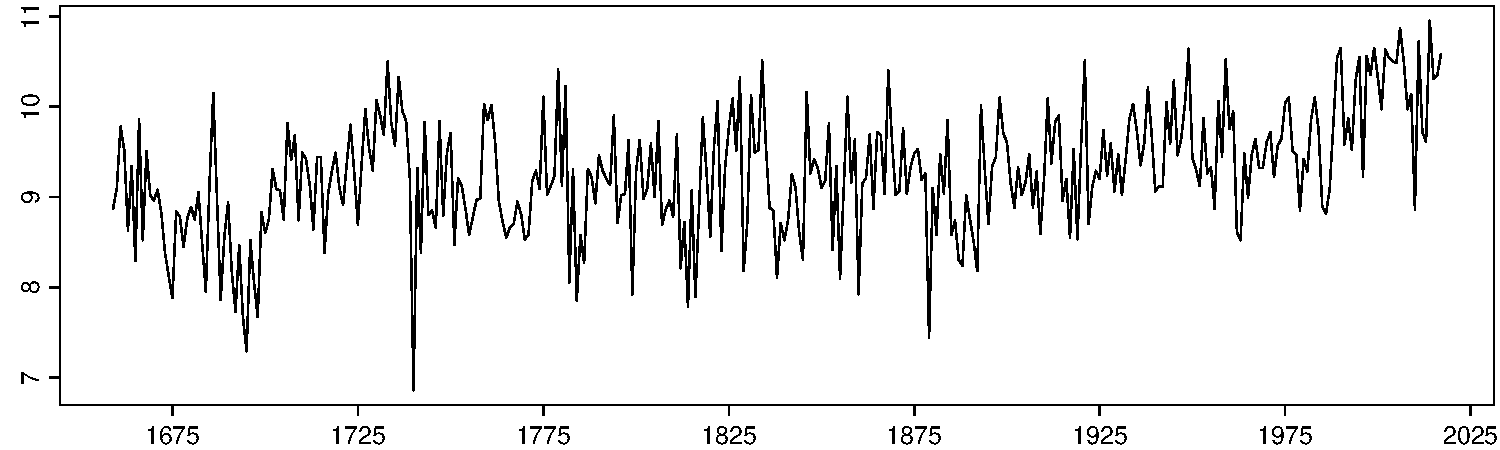
\includegraphics[width=0.9\textwidth]{Plots/temperature_data.pdf}
\vspace{0.15cm}

\caption{Yearly mean temperature in Central England from 1659 to 2017 measured in $^\circ$C.}\label{yearly_data}
\vspace{-0.15cm}
\end{figure}


Let us first have a closer look at the situation where a single time series is observed. In this case, practitioners are interested in questions such as the following: Does the observed time series have a trend at all? If so, which are the time regions where there is a strong trend? Is the trend decreasing or increasing in these regions? As an example, consider the time series plotted in Figure \ref{yearly_data} which shows the yearly mean temperature in Central England from 1659 to 2017. Climatologists are very much interested in analysing the trending behaviour of temperature time series like this; see e.g.\ \cite{Benner1999} and \cite{Rahmstorf2017}. Among other things, they would like to know whether there is an upward trend in the Central England mean temperature towards the end of the sample as visual inspection might suggest. In Section \ref{sec-test-shape}, we develop a statistical procedure to approach questions like this. Specifically, we construct a method to test the null hypothesis that there is no time trend in the data. Importantly, the proposed method does not only allow to test whether the null hypothesis of no trend is violated. It also allows to identify, with a pre-specified statistical confidence, time regions where there is some upward or downward movement in the trend. As regards the temperature time series in Figure \ref{yearly_data}, we can for example claim, with a statistical confidence of approximately 95\%, that there is some upward movement of the trend in the time period from about 1880 onwards. This is one of the results obtained from a detailed analysis of the time series as conducted in Section \ref{sec-data}. 


Let us now turn to the situation where multiple time series of the form \eqref{model2-intro} are observed. An important question in many applications is whether the time trends $m_i$ are the same for all $i$. When some of the trends are different, there may still be groups of time series with the same trend. In this case, it is often of interest to estimate the unknown groups from the data. In addition, when two trends $m_i$ and $m_j$ are not the same, it may also be relevant to know in which time regions they differ from each other. In Section \ref{sec-test-equality}, we construct statistical methods to approach these questions. In particular, we develop a test of the hypothesis that all time trends in model \eqref{model2-intro} are the same, that is, $m_1 = m_2 = \ldots = m_n$. Similar as before, our method does not only allow to test whether the null hypothesis is violated. It also allows to detect, with a given statistical confidence, which time trends are different and in which time regions they differ from each other. Based on our test method, we further construct an algorithm which clusters the observed time series into groups with the same trend. 
% Based on our test method, we further construct a clustering algorithm which estimates groups of time series with the same time trend.


We develop our methods and theory step by step in Sections \ref{sec-method}--\ref{sec-test-equality}. In Section \ref{sec-method}, we introduce our methods in the context of a simple baseline case. We in particular discuss the problem of testing the simple hypothesis $H_0: m = 0$ in model \eqref{model1-intro}. In Sections \ref{sec-test-shape} and \ref{sec-test-equality}, we adapt the methods and the theory to the test problems we are actually interested in. To construct our methods, we build on ideas from statistical multiscale testing as developed in \cite{ChaudhuriMarron1999,ChaudhuriMarron2000}, \cite{HallHeckman2000} and \cite{DuembgenSpokoiny2001} among others. Our test procedure for the simple hypothesis $H_0: m = 0$ in model \eqref{model1-intro} can be outlined as follows: In a first step, we set up statistics $\widehat{s}_T(u,h)$ to test the hypothesis $H_0(u,h)$ that $m = 0$ on the interval $[u-h,u+h]$. In a second step, we aggregate these statistics $\widehat{s}_T(u,h)$ for a wide range of intervals $[u-h,u+h]$. We thus construct a multiscale statistic which allows to test the hypothesis $H_0(u,h)$ simultaneously for many intervals $[u-h,u+h]$. A simple approach to aggregate the statistics $\widehat{s}_T(u,h)$ is to take their supremum $\sup_{(u,h) \in \mathcal{G_T}} |\widehat{s}_T(u,h)|$, where $\mathcal{G}_T$ denotes the set of points $(u,h)$ which are taken into account. As shown in the seminal work of \cite{DuembgenSpokoiny2001}, this approach is suboptimal in some sense. Following their lead, we define our multiscale statistic by $\widehat{\Psi}_T = \sup_{(u,h) \in \mathcal{G_T}} \{ |\widehat{s}_T(u,h)| - \lambda(h)\}$, where $\lambda(h)$ are additive correction terms. The idea behind this additively corrected supremum statistic is discussed in detail in Section \ref{sec-method}. 


In recent years, multiscale approaches have been developed for a variety of test problems. The general idea of all these approaches is to simultaneously consider a family of test statistics for a wide range of locations $u$ and scales or bandwidths $h$. This idea has been put to work in different ways, thus resulting in different multiscale test approaches. In the regression context, \cite{ChaudhuriMarron1999,ChaudhuriMarron2000} have developed the so-called SiZer method. 
% which has been extended in various directions; see for example \cite{KimMarron2006} and \cite{Huckemann2016} among others. 
\cite{HallHeckman2000} have constructed a multiscale test on monotonicity of a regression function. As already discussed above, \cite{DuembgenSpokoiny2001} have developed a multiscale approach which works with additively corrected supremum statistics. They derive theoretical results in the context of  a continuous Gaussian white noise model. Their theory can be extended in a fairly straightforward way to a nonparametric regression model $Y_t = m(t/T) + \varepsilon_t$ with i.i.d.\ Subgaussian errors $\varepsilon_t$. However, it is far from trivial to extend their theory to our setting, that is, to a nonparametric regression model $Y_t = m(t/T) + \varepsilon_t$ with a general weakly dependent error process $\{\varepsilon_t\}$. To derive our theoretical results, we come up with a proof strategy which is quite different from that of \cite{DuembgenSpokoiny2001}. This strategy is of interest in itself and may be applied to other multiscale test problems. It combines strong approximation results for dependent processes as developed in \cite{BerkesLiuWu2014} with anti-concentration bounds for Gaussian random vectors as derived in \cite{Chernozhukov2015}. The details are described in Section \ref{sec-method}.


\newpage
Whereas a number of multiscale tests for independent data have been developed in recent years, multiscale tests for dependent data are much rarer. Most notably, there are some extensions of the SiZer approach to a time series context. \cite{Rondonotti2004} and \cite{Rondonotti2007} have introduced dependent SiZer methods which can be regarded as an alternative to our multiscale test developed in Section \ref{sec-test-shape}. However, whereas their analysis is mainly methodological, we back up our multiscale test by a complete asymptotic theory which characterizes its size and power properties. \cite{Park2009} extend the SiZer approach to the problem of comparing multiple time trends. They provide some theory for the special case that the number of observed time series is $n=2$. In contrast to this, the theory for our multiscale method developed in Section \ref{sec-test-equality} is valid for any given number of time series $n$.


Besides the SiZer methods just discussed, there are several non-multiscale approaches to analyse nonparametric time trends. Tests on the presence and parametric form of a time trend have been developed in \cite{Dette1999} and \cite{ZhangWu2011} among others. Tests to compare nonparametric time trends have been constructed for example in \cite{DegrasWu2012} and \cite{ChenWu2018}, whereas \cite{Vogelsang2005} and \cite{Lyubchich2016} consider tests for comparing parametric time trends. One of the advantages of our multiscale approach is that it is very informative: It does not only allow to test whether the null hypothesis is violated. It also gives information on where violations occur. 
%In particular, it allows us to say, with a given statistical confidence, in which time regions there is an increase/decrease in the time trend under consideration, which time trends in our sample are different and in which time regions they differ. Our multiscale approach thus provides valuable additional information for practitioners. 
It thus provides valuable additional information for practitioners. 


%Our multiscale tests complement already existing tools for analysing nonparametric time trends. The test method developed in Section \ref{sec-test-shape} provides an alternative to dependent SiZer methods as introduced in \cite{Rondonotti2004} and \cite{Rondonotti2007}. Whereas the focus of these papers is mainly methodological, we back up our multiscale test by a complete asymptotic theory which characterizes its size and power properties. The multiscale test from Section \ref{sec-test-equality} is a valuable alternative to other procedures for testing equality of time trends. \cite{Park2009} extend the SiZer approach to the problem of comparing multiple time trends and provide some theory for the special case that the number of observed time series is $n=2$. Besides, there are several non-multiscale approaches to test for equality of time trends. \cite{Vogelsang2005} and \cite{Lyubchich2016}, for example, construct tests for comparing parametric time trends, whereas \cite{DegrasWu2012} and \cite{ChenWu2018} develop $L^2$-type tests for comparing nonparametric trends. One of the advantages of our multiscale approach is that it is very informative: It does not only allow to test whether the null hypothesis is violated or not. It also gives information on where violations occur, in particular, which time trends are different and in which time regions they differ. It thus provides valuable additional information for practitioners. 


We complement the theoretical analysis of the paper by a simulation study and two application examples in Sections \ref{sec-sim} and \ref{sec-data}. The simulation study investigates the finite sample properties of the test methods and the clustering algorithm from Sections \ref{sec-test-shape} and \ref{sec-test-equality}. In the first application example, we examine the temperature time series from Figure \ref{yearly_data} with the help of the methods developed in Section \ref{sec-test-shape}. In the second example, we analyse temperature time series measured at 25 different weather stations located in Great Britain. We in particular apply our procedure from Section \ref{sec-test-equality} to test whether the different time series have the same trend. 




\section{The model}\label{sec-model}


We now describe the two model settings in detail which were briefly outlined in the Introduction. The model for the test problems considered in Sections \ref{sec-method} and \ref{sec-test-shape} is as follows: We observe a single time series $\{Y_t: 1 \le t \le T \}$ of length $T$ which satisfies the model equation 
\begin{equation}\label{model1}
Y_t = m \Big( \frac{t}{T} \Big) + \varepsilon_t 
\end{equation}
for $1 \le t \le T$. Here, $m$ is an unknown nonparametric trend function defined on $[0,1]$ and $\{ \varepsilon_t: 1 \le t \le T \}$ is a zero-mean stationary error process. For simplicity, we restrict attention to equidistant design points $x_t = t/T$. However, our methods and theory can also be carried over to non-equidistant designs. The stationary error process $\{\varepsilon_t\}$ is assumed to have the following properties: 
\begin{enumerate}[label=(C\arabic*),leftmargin=1.05cm]

\item \label{C-err1} The variables $\varepsilon_t$ allow for the representation $\varepsilon_t = G(\ldots,\eta_{t-1},\eta_t)$, where $\eta_t$ are i.i.d.\ random variables and $G$ is a measurable function. 

\item \label{C-err2} It holds that $\| \varepsilon_t \|_q < \infty$ for some $q > 4$, where $\| \varepsilon_t \|_q = (\ex|\varepsilon_t|^q)^{1/q}$. 

\end{enumerate}
Following \cite{Wu2005}, we impose conditions on the dependence structure of the error process $\{\varepsilon_t\}$ in terms of the physical dependence measure $d_{t,q} = \| \varepsilon_t - \varepsilon_t^\prime \|_q$, where $\varepsilon_t^\prime = G(\ldots,\eta_{-1},\eta_0^\prime,\eta_1,\ldots,\eta_{t-1},\eta_t,\eta_{t+1},\ldots)$ with $\{\eta_t^\prime\}$ being an i.i.d.\ copy of $\{\eta_t\}$. In particular, we assume the following: 
\begin{enumerate}[label=(C\arabic*),leftmargin=1.05cm]
\setcounter{enumi}{2}

\item \label{C-err3} Define $\Theta_{t,q} = \sum\nolimits_{|s| \ge t} d_{s,q}$ for $t \ge 0$. It holds that 
\[ \Theta_{t,q} = O \big( t^{-\tau_q} (\log t)^{-A} \big), \]
where $A > \frac{2}{3} (1/q + 1 + \tau_q)$ and $\tau_q = \{q^2 - 4 + (q-2) \sqrt{q^2 + 20q + 4}\} / 8q$. 

\end{enumerate}
The conditions \ref{C-err1}--\ref{C-err3} are fulfilled by a wide range of stationary processes $\{\varepsilon_t\}$. As a first example, consider linear processes of the form $\varepsilon_t = \sum\nolimits_{i=0}^{\infty} c_i \eta_{t-i}$ with $\| \varepsilon_t \|_q < \infty$, where $c_i$ are absolutely summable coefficients and $\eta_t$ are i.i.d.\ innovations with $\ex[\eta_t] = 0$ and $\| \eta_t\|_q < \infty$. Trivially, \ref{C-err1} and \ref{C-err2} are fulfilled in this case. Moreover, if $|c_i| = O(\rho^i)$ for some $\rho \in (0,1)$, then \ref{C-err3} is easily seen to be satisfied as well. As a special case, consider an ARMA process $\{\varepsilon_t\}$ of the form $\varepsilon_t + \sum\nolimits_{i=1}^p a_i \varepsilon_{t-i} = \eta_t + \sum\nolimits_{j=1}^r b_j \eta_{t-j}$  with $\| \varepsilon_t \|_q < \infty$, where $a_1,\ldots,a_p$ and $b_1,\ldots,b_r$ are real-valued parameters. As before, we let $\eta_t$ be i.i.d.\ innovations with $\ex[\eta_t] = 0$ and $\| \eta_t\|_q < \infty$. Moreover, as usual, we suppose that the complex polynomials $A(z) = 1 + \sum\nolimits_{j=1}^p a_jz^j$ and $B(z) = 1 + \sum\nolimits_{j=1}^r b_jz^j$ do not have any roots in common. If $A(z)$ does not have any roots inside the unit disc, then the ARMA process $\{ \varepsilon_t \}$ is stationary and causal. Specifically, it has the representation $\varepsilon_t = \sum\nolimits_{i=0}^{\infty} c_i \eta_{t-i}$ with $|c_i| = O(\rho^i)$ for some $\rho \in (0,1)$, implying that \ref{C-err1}--\ref{C-err3} are fulfilled. The results in \cite{WuShao2004} show that condition \ref{C-err3} (as well as the other two conditions) is not only fulfilled for linear time series processes but also for a variety of non-linear processes. 


The model setting for the test problem analysed in Section \ref{sec-test-equality} is closely related to the setting discussed above. The main difference is that we observe multiple rather than only one time series. In particular, we observe time series $\mathcal{Y}_i = \{Y_{it}: 1 \le t \le T \}$ of length $T$ for $1 \le i \le n$. Each time series $\mathcal{Y}_i$ satisfies the model equation \begin{equation}\label{model2}
Y_{it} = m_i \Big( \frac{t}{T} \Big) + \alpha_i + \varepsilon_{it} 
\end{equation}
for $1 \le t \le T$, where $m_i$ is an unknown nonparametric trend function defined on $[0,1]$, $\alpha_i$ is a (deterministic or random) intercept term and $\mathcal{E}_i = \{ \varepsilon_{it}: 1 \le t \le T \}$ is a zero-mean stationary error process. For identification, we normalize the functions $m_i$ such that $\int_0^1 m_i(u) du = 0$ for all $1 \le i \le n$. The term $\alpha_i$ can also be regarded as an additional error component. In the econometrics literature, it is commonly called a fixed effect error term. It can be interpreted as capturing unobserved characteristics of the time series $\mathcal{Y}_i$ which remain constant over time. We allow the error terms $\alpha_i$ to be dependent across $i$ in an arbitrary way. Hence, by including them in model equation \eqref{model2}, we allow the $n$ time series $\mathcal{Y}_i$ in our sample to be correlated with each other. Whereas the terms $\alpha_i$ may be correlated, the error processes $\mathcal{E}_i$ are assumed to be independent across $i$. In addition, each process $\mathcal{E}_i$ is supposed to satisfy the conditions \ref{C-err1}--\ref{C-err3}. Finally note that throughout the paper, we restrict attention to the case where the number of time series $n$ in model \eqref{model2} is bounded. It is however possible to extend our theoretical results to the case where $n$ slowly grows with the sample size $T$.



\section{The multiscale method}\label{sec-method}


In this section, we introduce our multiscale test method and the underlying theory for the simple hypothesis $H_0: m = 0$ in model \eqref{model1}. As we will see in Sections \ref{sec-test-shape} and \ref{sec-test-equality}, both the method and the theory for this simple case can be easily adapted to more interesting test problems, in particular to the test problems discussed in the Introduction. 
%Both the method and the theory for this simple case can be easily adapted to more interesting test problems as we will see in Sections \ref{sec-test-shape} and \ref{sec-test-equality}. 
%The discussion can be regarded as providing a blueprint of our multiscale methods and the underlying theory, which is ready to adapt to more advanced test problems. 


\subsection{Construction of the test statistic}\label{subsec-method-stat}


To construct a multiscale test statistic for the hypothesis $H_0: m = 0$ in model \eqref{model1}, we consider the kernel averages
\begin{equation*}
\widehat{\psi}_T(u,h) = \sum\limits_{t=1}^T w_{t,T}(u,h) Y_t, 
\end{equation*}
where $w_{t,T}(u,h)$ is a kernel weight with $u \in [0,1]$ and the bandwidth parameter $h$. In order to avoid boundary issues, we work with a local linear weighting scheme. We in particular set 
\begin{equation}\label{weights}
w_{t,T}(u,h) = \frac{\Lambda_{t,T}(u,h)}{ \{\sum\nolimits_{t=1}^T \Lambda_{t,T}^2(u,h)\}^{1/2} }, 
\end{equation}
where
\[ \Lambda_{t,T}(u,h) = K\Big(\frac{\frac{t}{T}-u}{h}\Big) \Big[ S_{T,2}(u,h) - S_{T,1}(u,h) \Big(\frac{\frac{t}{T}-u}{h}\Big) \Big], \]
$S_{T,\ell}(u,h) = (Th)^{-1} \sum\nolimits_{t=1}^T K(\frac{\frac{t}{T}-u}{h}) (\frac{\frac{t}{T}-u}{h})^\ell$ for $\ell = 0,1,2$ and $K$ is a kernel function with the following properties: 
\begin{enumerate}[label=(C\arabic*),leftmargin=1.05cm]
\setcounter{enumi}{3}
\item \label{C-ker} The kernel $K$ is non-negative, symmetric about zero and integrates to one. Moreover, it has compact support $[-1,1]$ and is Lipschitz continuous, that is, $|K(v) - K(w)| \le C |v-w|$ for any $v,w \in \reals$ and some constant $C > 0$. 
\end{enumerate} 
Alternatively to the local linear weights defined in \eqref{weights}, we could also work with local constant weights which are defined analogously with $\Lambda_{t,T}(u,h) = K(\frac{\frac{t}{T}-u}{h})$. We however prefer to use local linear weights as these have superior theoretical properties at the boundary.  


The kernel average $\widehat{\psi}_T(u,h)$ is a local average of the observations $Y_1,\ldots,Y_T$ which gives positive weight only to data points $Y_t$ with $t/T \in [u-h,u+h]$. Hence, only observations $Y_t$ with $t/T$ close to the location $u$ are taken into account, the amount of localization being determined by the bandwidth $h$. With the weights defined in \eqref{weights}, the kernel average $\widehat{\psi}_T(u,h)$ is nothing else than a rescaled local linear estimator of $m(u)$ with bandwidth $h$. The weights are chosen such that in the case of independent error terms $\varepsilon_t$, $\var(\widehat{\psi}_T(u,h)) = \sigma^2$ for any location $u$ and bandwidth $h$, where $\sigma^2 = \var(\varepsilon_t)$. In the more general case that the error terms satisfy the weak dependence conditions from Section \ref{sec-model}, it holds that $\var(\widehat{\psi}_T(u,h)) = \sigma^2 + o(1)$ for any location $u$ and any bandwidth $h$ with $h \rightarrow 0$ and $Th \rightarrow \infty$, where $\sigma^2 = \sum\nolimits_{\ell=-\infty}^{\infty} \cov(\varepsilon_0, \varepsilon_{\ell})$ is the long-run variance of the error terms. Hence, the statistics $\widehat{\psi}_T(u,h)$ have approximately the same variance across $u$ and $h$ for sufficiently large sample sizes $T$. In what follows, we consider normalized versions $\widehat{\psi}_T(u,h)/\widehat{\sigma}$ of the kernel averages $\widehat{\psi}_T(u,h)$, where $\widehat{\sigma}^2$ is an estimator of the long-run error variance $\sigma^2$. The problem of estimating $\sigma^2$ is discussed in detail in Section \ref{sec-error-var}. There, we construct estimators $\widehat{\sigma}^2$ with the property that $\widehat{\sigma}^2 = \sigma^2 + O_p(1/\sqrt{T})$ under appropriate conditions. For the time being, we suppose that $\widehat{\sigma}^2$ is an estimator with reasonable theoretical properties. We in particular assume that $\widehat{\sigma}^2 = \sigma^2 + o_p(\rho_T)$ with $\rho_T = o(1/\log T)$. The convergence rate $\rho_T$ is thus allowed to be much slower than $1/\sqrt{T}$. 


Our multiscale statistic combines the kernel averages $\widehat{\psi}_T(u,h)$ for a wide range of different locations $u$ and bandwidths or scales $h$. Specifically, it is defined as
\begin{equation}\label{multiscale-stat}
\widehat{\Psi}_T = \max_{(u,h) \in \mathcal{G}_T} \Big\{ \Big|\frac{\widehat{\psi}_T(u,h)}{\widehat{\sigma}}\Big| - \lambda(h) \Big\}, 
\end{equation} 
where $\lambda(h) = \sqrt{2 \log \{ 1/(2h) \}}$ and $\mathcal{G}_T$ is the set of points $(u,h)$ that are taken into consideration. The details on the set $\mathcal{G}_T$ are discussed below. As can be seen, the statistic $\widehat{\Psi}_T$ does not simply aggregate the individual statistics $\widehat{\psi}_T(u,h)/\widehat{\sigma}$ by taking the supremum over all points $(u,h) \in \mathcal{G}_T$ as in more traditional multiscale approaches. We rather follow the approach pioneered by \cite{DuembgenSpokoiny2001} and subtract the additive correction term $\lambda(h)$ from the statistics $\widehat{\psi}_T(u,h)/\widehat{\sigma}$ that correspond to the bandwidth level $h$. To see the heuristic idea behind the additive correction $\lambda(h)$, consider for a moment the uncorrected statistic
\[ \widehat{\Psi}_{T,\text{uncorrected}} = \max_{(u,h) \in \mathcal{G}_T} \Big|\frac{\widehat{\psi}_T(u,h)}{\widehat{\sigma}}\Big| \]
and suppose that the null hypothesis $H_0: m = 0$ holds true. For simplicity, assume that the errors $\varepsilon_t$ are i.i.d.\ normally distributed and neglect the estimation error in $\widehat{\sigma}$, that is, set $\widehat{\sigma} = \sigma$. Moreover, suppose that the set $\mathcal{G}_T$ only consists of the points $(u_k,h_\ell) = ((2k - 1)h_\ell,h_\ell)$ with $k = 1,\ldots,\lfloor 1/2h_\ell \rfloor$ and $\ell = 1,\ldots,L$. In this case, we can write
\[ \widehat{\Psi}_{T,\text{uncorrected}} = \max_{1 \le \ell \le L} \max_{1 \le k \le \lfloor 1/2h_\ell \rfloor} \Big|\frac{\widehat{\psi}_T(u_k,h_\ell)}{\sigma}\Big|. \]
Under our simplifying assumptions, the statistics $\widehat{\psi}_T(u_k,h_\ell)/\sigma$ with $k = 1,\ldots,\lfloor 1/2h_\ell \rfloor$ are independent and standard normal for any given bandwidth $h_\ell$. Since the maximum over $\lfloor 1/2h \rfloor$ independent standard normal random variables is $\lambda(h) + o_p(1)$ as $h \rightarrow 0$, we obtain that $\max_{k} \widehat{\psi}_T(u_k,h_\ell)/\sigma$ is approximately of size $\lambda(h_\ell)$ for small bandwidths $h_\ell$. As $\lambda(h) \rightarrow \infty$ for $h \rightarrow 0$, this implies that $\max_{k} \widehat{\psi}_T(u_k,h_\ell)/\sigma$ tends to be much larger in size for small than for large bandwidths $h_\ell$. As a result, the stochastic behaviour of the uncorrected statistic $\widehat{\Psi}_{T,\text{uncorrected}}$ tends to be dominated by the statistics $\widehat{\psi}_T(u_k,h_\ell)$ corresponding to small bandwidths $h_\ell$. The additively corrected statistic $\widehat{\Psi}_T$, in contrast, puts the statistics $\widehat{\psi}_T(u_k,h_\ell)$ corresponding to different bandwidths $h_\ell$ on a more equal footing, thus counteracting the dominance of small bandwidth values. 


The multiscale statistic $\widehat{\Psi}_T$ simultaneously takes into account all locations $u$ and bandwidths $h$ with $(u,h) \in \mathcal{G}_T$. Throughout the paper, we suppose that $\mathcal{G}_T$ is some subset of $\mathcal{G}_T^{\text{full}} = \{ (u,h): u = t/T \text{ for some } 1 \le t \le T \text{ and } h \in [h_{\min},h_{\max}] \}$, where $h_{\min}$ and $h_{\max}$ denote some minimal and maximal bandwidth value, respectively. For our theory to work, we require the following conditions to hold:
\begin{enumerate}[label=(C\arabic*),leftmargin=1.05cm]
\setcounter{enumi}{4}

\item \label{C-grid} $|\mathcal{G}_T| = O(T^\theta)$ for some arbitrarily large but fixed constant $\theta > 0$, where $|\mathcal{G}_T|$ denotes the cardinality of $\mathcal{G}_T$. 

\item \label{C-h} $h_{\min} \gg T^{-(1-\frac{2}{q})} \log T$, that is, $h_{\min} / \{ T^{-(1-\frac{2}{q})} \log T \} \rightarrow \infty$ with $q > 4$ defined in \ref{C-err2} and $h_{\max} = o(1)$.

\end{enumerate}
According to \ref{C-grid}, the number of points $(u,h)$ in $\mathcal{G}_T$ should not grow faster than $T^\theta$ for some arbitrarily large but fixed $\theta > 0$. This is a fairly weak restriction as it allows the set $\mathcal{G}_T$ to be extremely large as compared to the sample size $T$. For example, we may work with the set 
\begin{align*}
\mathcal{G}_T = \big\{ & (u,h): u = t/T \text{ for some } 1 \le t \le T \text{ and } h \in [h_{\min},h_{\max}] \\ & \text{ with } h = t/T \text{ for some } 1 \le t \le T  \big\},
\end{align*}
which contains more than enough points $(u,h)$ for most practical applications. Condition \ref{C-h} imposes some restrictions on the minimal and maximal bandwidths $h_{\min}$ and $h_{\max}$. These conditions are fairly weak, allowing us to choose the bandwidth window $[h_{\min},h_{\max}]$ extremely large. In particular, we can choose the minimal bandwidth $h_{\min}$ to be of the order $T^{-1/2}$ for any $q > 4$, which means that we can let $h_{\min}$ converge to $0$ very quickly. Moreover, the maximal bandwidth $h_{\max}$ is allowed to converge to $0$ arbitrarily slowly, which implies that we can pick it very large.


\subsection{The test procedure}\label{subsec-method-test}


In order to formulate a test for the hypothesis $H_0: m = 0$, we still need to specify a critical value. To do so, we define the statistic
\begin{equation}\label{Phi-statistic}
\Phi_T = \max_{(u,h) \in \mathcal{G}_T} \Big\{ \Big|\frac{\phi_T(u,h)}{\sigma}\Big| - \lambda(h) \Big\},
\end{equation} 
where $\phi_T(u,h) = \sum\nolimits_{t=1}^T w_{t,T}(u,h) \, \sigma Z_t$ and $Z_t$ are independent standard normal random variables. The statistic $\Phi_T$ can be regarded as a Gaussian version of the test statistic $\widehat{\Psi}_T$ under the null hypothesis $H_0$. Let $q_T(\alpha)$ be the $(1-\alpha)$-quantile of $\Phi_T$. Importantly, the quantile $q_T(\alpha)$ can be computed by Monte Carlo simulations and can thus be regarded as known. Our multiscale test of the hypothesis $H_0: m = 0$ is now defined as follows: For a given significance level $\alpha \in (0,1)$, we reject $H_0$ if $\widehat{\Psi}_T > q_T(\alpha)$. 


\subsection{Theoretical properties of the test}\label{subsec-method-theo}


In order to examine the theoretical properties of our multiscale test, we introduce the statistic 
\begin{align}
\widehat{\Phi}_T 
% & = \max_{(u,h) \in \mathcal{G}_T} \Big\{ \Big| \frac{\widehat{\psi}_T(u,h) - \ex \widehat{\psi}_T(u,h)}{\widehat{\sigma}} \Big| - \lambda(h) \Big\} \nonumber \\
 & = \max_{(u,h) \in \mathcal{G}_T} \Big\{ \Big| \frac{\widehat{\phi}_T(u,h)}{\widehat{\sigma}} \Big| - \lambda(h) \Big\} \label{Phi-hat-statistic}
\end{align}
with $\widehat{\phi}_T(u,h) = \widehat{\psi}_T(u,h) - \ex [\widehat{\psi}_T(u,h)] = \sum\nolimits_{t=1}^T w_{t,T}(u,h) \varepsilon_t$. According to the following theorem, the (known) quantile $q_T(\alpha)$ of $\Phi_T$ defined in Section \ref{subsec-method-test} can be used as a proxy for the $(1-\alpha)$-quantile of the statistic $\widehat{\Phi}_T$.
\begin{theorem}\label{theo-stat}
Let \ref{C-err1}--\ref{C-h} be fulfilled and assume that $\widehat{\sigma}^2 = \sigma^2 + o_p(\rho_T)$ with $\rho_T = o(1/\log T)$. Then 
\[ \pr \big( \widehat{\Phi}_T \le q_T(\alpha) \big) = (1 - \alpha) + o(1). \]
\end{theorem}
A full proof of Theorem \ref{theo-stat} is given in the Appendix. 
%We here shortly outline the proof strategy, which is of broader interest as it can potentially be applied in the context of a variety of other statistical multiscale problems. The strategy splits up into two main steps: 
We here shortly outline the proof strategy, which splits up into two main steps. In the first, we replace the statistic $\widehat{\Phi}_T$ for each $T \ge 1$ by a statistic $\widetilde{\Phi}_T$ with the same distribution as $\widehat{\Phi}_T$ and the property that 
\begin{equation}\label{eq-theo-stat-strategy-step1}
\big| \widetilde{\Phi}_T - \Phi_T \big| = o_p(\delta_T),
\end{equation}
where $\delta_T = o(1)$ and the Gaussian statistic $\Phi_T$ is defined in Section \ref{subsec-method-test}. We thus replace the statistic $\widehat{\Phi}_T$ by an identically distributed version which is close to a Gaussian statistic whose distribution is known. To do so, we make use of strong approximation theory for dependent processes as derived in \cite{BerkesLiuWu2014}. In the second step, we show that 
\begin{equation}\label{eq-theo-stat-strategy-claim}
\sup_{x \in \reals} \big| \pr(\widetilde{\Phi}_T \le x) - \pr(\Phi_T \le x) \big| = o(1), 
\end{equation}
which immediately implies the statement of Theorem \ref{theo-stat}. Importantly, the convergence result \eqref{eq-theo-stat-strategy-step1} is not sufficient for establishing \eqref{eq-theo-stat-strategy-claim}. Put differently, the fact that $\widetilde{\Phi}_T$ can be approximated by $\Phi_T$ in the sense that $\widetilde{\Phi}_T - \Phi_T = o_p(\delta_T)$ does not imply that the distribution of $\widetilde{\Phi}_T$ is close to that of $\Phi_T$ in the sense of \eqref{eq-theo-stat-strategy-claim}. For \eqref{eq-theo-stat-strategy-claim} to hold, we additionally require the distribution of $\Phi_T$ to have some sort of continuity property. Specifically, we prove that 
\begin{equation}\label{eq-theo-stat-strategy-step2}
\sup_{x \in \reals} \pr \big( |\Phi_T - x| \le \delta_T \big) = o(1),
\end{equation}
which says that $\Phi_T$ does not concentrate too strongly in small regions of the form $[x-\delta_T,x+\delta_T]$. The main tool for verifying \eqref{eq-theo-stat-strategy-step2} are anti-concentration results for Gaussian random vectors as derived in \cite{Chernozhukov2015}. The claim \eqref{eq-theo-stat-strategy-claim} can be proven by combining \eqref{eq-theo-stat-strategy-step1} and \eqref{eq-theo-stat-strategy-step2}, which in turn yields Theorem \ref{theo-stat}. 


With the help of Theorem \ref{theo-stat}, we can investigate the theoretical properties of our multiscale test. The first result is an immediate consequence of Theorem \ref{theo-stat}. It says that the test has the correct (asymptotic) size. 
\begin{prop}\label{prop-test-1}
Let the conditions of Theorem \ref{theo-stat} be satisfied. Under the null hypothesis $H_0: m = 0$, it holds that 
\[ \pr \big( \widehat{\Psi}_T \le q_T(\alpha) \big) = (1 - \alpha) + o(1). \]
\end{prop}
The second result characterizes the power of the multiscale test against local alternatives. To formulate it, we consider any sequence of functions $m = m_T$ with the following property: There exists $(u,h) \in \mathcal{G}_T$ with $[u-h,u+h] \subseteq [0,1]$ such that 
\begin{equation}\label{loc-alt}
m_T(w) \ge c_T \sqrt{\frac{\log T}{Th}} \quad \text{for all } w \in [u-h,u+h], 
\end{equation}
where $\{c_T\}$ is any sequence of positive numbers with $c_T \rightarrow \infty$. Alternatively to \eqref{loc-alt}, we may also assume that $-m_T(w) \ge c_T \sqrt{\log T/(Th)}$ for all $w \in [u-h,u+h]$. According to the following result, our test has asymptotic power $1$ against local alternatives of the form \eqref{loc-alt}. 
\begin{prop}\label{prop-test-2}
Let the conditions of Theorem \ref{theo-stat} be satisfied and consider any sequence of functions $m_T$ with the property \eqref{loc-alt}. Then 
\[ \pr \big( \widehat{\Psi}_T \le q_T(\alpha) \big) = o(1). \]
\end{prop}
The proof of Proposition \ref{prop-test-2} can be found in the Appendix. To formulate the next result, we define 
\[ \Pi_T = \big\{ I_{u,h} = [u-h,u+h]: (u,h) \in \mathcal{A}_T \big\} \]
with 
\[ \mathcal{A}_T = \Big\{ (u,h) \in \mathcal{G}_T: \Big|\frac{\widehat{\psi}_T(u,h)}{\widehat{\sigma}}\Big| - \lambda(h) > q_T(\alpha) \Big\}. \]
$\Pi_T$ is the collection of intervals $I_{u,h} = [u-h,u+h]$ for which the (corrected) test statistic $|\widehat{\psi}_T(u,h)/\widehat{\sigma}| - \lambda(h)$ lies above the critical value $q_T(\alpha)$. With this notation at hand, we consider the event 
\[ E_T = \Big\{ \forall I_{u,h} \in \Pi_T: m(v) \ne 0 \text{ for some } v \in I_{u,h} = [u-h,u+h] \Big\}. \]
This is the event that the null hypothesis is violated on all intervals $I_{u,h}$ for which the (corrected) test statistic $|\widehat{\psi}_T(u,h)/\widehat{\sigma}| - \lambda(h)$ is above the critical value $q_T(\alpha)$. We can make the following formal statement about the event $E_T$ whose proof is given in the Appendix. 
\begin{prop}\label{prop-test-3}
Under the conditions of Theorem \ref{theo-stat}, it holds that  
\[ \pr \big( E_T \big) \ge (1-\alpha) + o(1). \] 
\end{prop}
According to Proposition \ref{prop-test-3}, our test procedure allows to make uniform confidence statements of the following form: With (asymptotic) probability $\ge (1-\alpha)$, the null hypothesis $H_0: m = 0$ is violated on all intervals $I_{u,h} \in \Pi_T$. Hence, our multiscale test does not only allow to check whether the null hypothesis is violated. It also allows to identify regions where violations occur with a pre-specified level of confidence. 
 

The statement of Proposition \ref{prop-test-3} suggests to graphically present the results of our multiscale test by plotting the intervals $I_{u,h} \in \Pi_T$, that is, by plotting the intervals where (with asymptotic confidence $\ge 1-\alpha$) our test detects a violation of the null hypothesis. The drawback of this graphical presentation is that the number of intervals in $\Pi_T$ is often quite large. To obtain a better graphical summary of the results, we replace $\Pi_T$ by a subset $\Pi_T^{\min}$ which is constructed as follows: As in \cite{Duembgen2002}, we call an interval $I_{u,h} \in \Pi_T$ minimal if there is no other interval $I_{u^\prime,h^\prime} \in \Pi_T$ with $I_{u^\prime,h^\prime} \subset I_{u,h}$. Let $\Pi_T^{\min}$ be the set of all minimal intervals in $\Pi_T$ and define the event 
\[ E_T^{\min} = \Big\{ \forall I_{u,h} \in \Pi_T^{\min}: m(v) \ne 0 \text{ for some } v \in I_{u,h} = [u-h,u+h] \Big\}. \]
It is easily seen that $E_T = E_T^{\min}$. Hence, by Proposition \ref{prop-test-3}, it holds that 
\[ \pr \big(E_T^{\min}\big) \ge (1-\alpha) + o(1). \] 
This suggests to plot the minimal intervals in $\Pi_T^{\min}$ rather than the whole collection of intervals $\Pi_T$ as a graphical summary of the test results. We in particular use this way of presenting the test results in our application examples of Section \ref{sec-data}. 



\section{Testing for the presence of a time trend}\label{sec-test-shape}


In what follows, we construct a multiscale test for the null hypothesis that the trend function $m$ in model \eqref{model1} is constant. To achieve this, we adapt the methodology developed in Section \ref{sec-method}. Importantly, the resulting multiscale procedure does not only allow to test whether the null hypothesis is violated. As we will see, it also allows to identify, with a pre-specified statistical confidence, time regions where violations occur. Put differently, it allows to identify, with a given confidence, intervals $I_{u,h} = [u-h,u+h]$ where $m$ is not constant over time.
%, that is, where there is an increase/decrease in the time trend $m$. 
It thus provides information on where the time trend is increasing/decreasing, which is important knowledge in many applications. 


\subsection{Construction of the test statistic}\label{subsec-test-shape-stat}


Throughout the section, we suppose that the trend $m$ is continuously differentiable. The null hypothesis that $m$ is constant can be formulated as $H_0: m^\prime = 0$, where $m^\prime$ denotes the first derivative of $m$. To construct a test statistic for the hypothesis $H_0$, we proceed analogously as in Section \ref{subsec-method-stat}. To start with, we introduce the kernel averages 
\begin{equation*}
\widehat{\psi}_T^\prime(u,h) = \sum\limits_{t=1}^T w_{t,T}^\prime(u,h) Y_t, 
\end{equation*}
where the kernel weights $w_{t,T}^\prime(u,h)$ are given by 
\begin{equation}\label{weights-deriv}
w_{t,T}^\prime(u,h) = \frac{\Lambda_{t,T}^\prime(u,h)}{ \{\sum\nolimits_{t=1}^T \Lambda_{t,T}^\prime(u,h)^2 \}^{1/2} } 
\end{equation}
with
\[ \Lambda_{t,T}^\prime(u,h) = K\Big(\frac{\frac{t}{T}-u}{h}\Big) \Big[ S_{T,0}(u,h) \Big(\frac{\frac{t}{T}-u}{h}\Big) - S_{T,1}(u,h) \Big]. \]
Here, $S_{T,\ell}(u,h)$ is defined as in Section \ref{subsec-method-stat} and $K$ is a kernel function which satisfies \ref{C-ker}. The kernel average $\widehat{\psi}_T^\prime(u,h)$ is a rescaled version of the local linear estimator of the derivative $m^\prime(u)$ with bandwidth $h$. Alternatively to the local linear weights defined in \eqref{weights-deriv}, we could employ the weights $w_{t,T}^\prime(u,h) = K^\prime( \frac{u - \frac{t}{T}}{h} )/ \{ \sum\nolimits_{t=1}^T  K^\prime( \frac{u - \frac{t}{T}}{h} )^2 \}^{1/2}$, where the kernel function $K$ is assumed to be differentiable and $K^\prime$ is its derivative. To avoid boundary problems, we however work with the local linear weights from \eqref{weights-deriv} throughout the paper. Our multiscale statistic is defined as 
\[ \widehat{\Psi}_T^\prime = \max_{(u,h) \in \mathcal{G}_T} \Big\{ \Big|\frac{\widehat{\psi}_T^\prime(u,h)}{\widehat{\sigma}}\Big| - \lambda(h) \Big\}, \] 
where $\lambda(h) = \sqrt{2 \log \{ 1/(2h) \}}$ and the set $\mathcal{G}_T$ has been introduced in Section \ref{subsec-method-stat}. As can be seen, the statistic $\widehat{\Psi}_T^\prime$ is very similar to that from Section \ref{sec-method}. Only the kernel averages $\widehat{\psi}_T^\prime(u,h)$ have a somewhat different form. 


\subsection{The test procedure}\label{subsec-test-shape-test}


As in Section \ref{subsec-method-test}, we define a Gaussian version $\Phi_T^\prime$ of the test statistic $\widehat{\Psi}_T^\prime$ under the null hypothesis $H_0$ by
\[ \Phi_T^\prime = \max_{(u,h) \in \mathcal{G}_T} \Big\{ \Big|\frac{\phi_T^\prime(u,h)}{\sigma}\Big| - \lambda(h) \Big\}, \] 
where $\phi_T^\prime(u,h) = \sum\nolimits_{t=1}^T w_{t,T}^\prime(u,h) \, \sigma Z_t$ and $Z_t$ are independent standard normal random variables. Denoting the $(1-\alpha)$-quantile of $\Phi_T^\prime$ by $q_T^\prime(\alpha)$, our multiscale test of the hypothesis $H_0$: $m^\prime = 0$ is defined as follows: For a given significance level $\alpha \in (0,1)$, we reject $H_0$ if $\widehat{\Psi}_T^\prime > q_T^\prime(\alpha)$. 


\subsection{Theoretical properties of the test}\label{subsec-test-shape-theo}


The theoretical analysis parallels that of Section \ref{subsec-method-theo}. We first investigate the theoretical properties of the auxiliary statistic 
\begin{align*}
\widehat{\Phi}_T^\prime = \max_{(u,h) \in \mathcal{G}_T} \Big\{ \Big| \frac{\widehat{\phi}_T^\prime(u,h)}{\widehat{\sigma}} \Big| - \lambda(h) \Big\}, 
\end{align*}
where $\widehat{\phi}_T^\prime(u,h) = \sum_{t=1}^T w_{t,T}^\prime(u,h) \varepsilon_t$. The following result adapts Theorem \ref{theo-stat} to our current test problem. 
\begin{theorem}\label{theo-stat-shape}
Let \ref{C-err1}--\ref{C-h} be fulfilled and assume that $\widehat{\sigma}^2 = \sigma^2 + o_p(\rho_T)$ with $\rho_T = o(1/\log T)$. Then
\[ \pr \big( \widehat{\Phi}_T^\prime \le q_T^\prime(\alpha) \big) = (1 - \alpha) + o(1). \]
\end{theorem}
The proof of Theorem \ref{theo-stat-shape} is essentially the same as that of Theorem \ref{theo-stat} and thus omitted. With the help of Theorem \ref{theo-stat-shape}, we can derive the following theoretical properties of our multiscale test. 
\newpage
\begin{prop}\label{prop-test-shape-1}
Let the conditions of Theorem \ref{theo-stat-shape} be satisfied. 
\begin{enumerate}[label=(\alph*),leftmargin=0.75cm]
\item Under the null hypothesis $H_0$, it holds that 
\[ \pr \big( \widehat{\Psi}_T^\prime \le q_T^\prime(\alpha) \big) = (1 - \alpha) + o(1). \]
\item Consider any sequence of functions $m = m_T$ with the following property: There exists $(u,h) \in \mathcal{G}_T$ with $[u-h,u+h] \subseteq [0,1]$ such that $m_T^\prime(w) \ge c_T \sqrt{\log T/(Th^3)}$ for all $w \in [u-h,u+h]$ or $-m_T^\prime(w) \ge c_T \sqrt{\log T/(Th^3)}$ for all $w \in [u-h,u+h]$, where $\{c_T\}$ is any sequence of positive numbers with $c_T \rightarrow \infty$. Then 
\[ \pr \big( \widehat{\Psi}_T^\prime \le q_T^\prime(\alpha) \big) = o(1). \]
\end{enumerate}
\end{prop}
Part (a) of Proposition \ref{prop-test-shape-1} is a simple consequence of Theorem \ref{theo-stat-shape}. Part (b) can be proven by similar arguments as Proposition \ref{prop-test-2}. The details are given in the Supplementary Material. Taken together, the two parts of Proposition \ref{prop-test-shape-1} show that our multiscale test has the correct (asymptotic) size and that it is able to detect certain local alternatives with probability tending to $1$. We next consider the events
\begin{align*}
E_T^+ & = \Big\{ \forall I_{u,h} \in \Pi_T^+: m^\prime(v) > 0 \text{ for some } v \in I_{u,h} = [u-h,u+h] \Big\} \\
E_T^- & = \Big\{ \forall I_{u,h} \in \Pi_T^-: m^\prime(v) < 0 \text{ for some } v \in I_{u,h} = [u-h,u+h] \Big\},
\end{align*}
where the sets $\Pi_T^+$ and $\Pi_T^-$ are given by
\begin{align*}
\Pi_T^+ & = \big\{ I_{u,h} = [u-h,u+h]: (u,h) \in \mathcal{A}_T^+ \text{ and } I_{u,h} \subseteq [0,1] \big\} \\
\Pi_T^- & = \big\{ I_{u,h} = [u-h,u+h]: (u,h) \in \mathcal{A}_T^- \text{ and } I_{u,h} \subseteq [0,1] \big\} 
\end{align*}
with 
\begin{align*}
\mathcal{A}_T^+ & = \Big\{ (u,h) \in \mathcal{G}_T: \frac{\widehat{\psi}_T^\prime(u,h)}{\widehat{\sigma}} > q_T^\prime(\alpha) + \lambda(h) \Big\} \\ 
\mathcal{A}_T^- & = \Big\{ (u,h) \in \mathcal{G}_T: -\frac{\widehat{\psi}_T^\prime(u,h)}{\widehat{\sigma}} > q_T^\prime(\alpha) + \lambda(h) \Big\}. 
\end{align*}
$E_T^+$ is the event that for each interval $I_{u,h} \in \Pi_T^+$, there is a subset $J_{u,h} \subseteq I_{u,h}$ with $m$ being an increasing function on $J_{u,h}$. An analogous description applies to the event $E_T^-$. The following result shows that the events $E_T^+$ and $E_T^-$ occur with asymptotic probability $\ge 1-\alpha$. 
\begin{prop}\label{prop-test-shape-2}
Under the conditions of Theorem \ref{theo-stat-shape}, it holds that  
\begin{align*}
\pr \big( E_T^+ \big) & \ge (1-\alpha) + o(1) \\
\pr \big( E_T^- \big) & \ge (1-\alpha) + o(1). 
\end{align*}
\end{prop}
The proof of Proposition \ref{prop-test-shape-2} parallels that of Proposition \ref{prop-test-3}. The details are provided in the Supplementary Material. The statement of Proposition \ref{prop-test-shape-2} can be summarized as follows: With asymptotic probability $\ge 1-\alpha$, there is a subset $J_{u,h} \subseteq I_{u,h}$ for each interval $I_{u,h} \in \Pi_T^+$ such that $m$ is an increasing function on $J_{u,h}$. Put differently, with asymptotic probability $\ge 1- \alpha$, the trend $m$ is increasing on some part of the interval $I_{u,h}$ for any $I_{u,h} \in \Pi_T^+$. An analogous statement holds for the intervals in the set $\Pi_T^-$. Our multiscale procedure thus allows to identify, with a pre-specified confidence, time regions where there is an increase/decrease in the time trend $m$. 


We close the section with some additional remarks on Proposition \ref{prop-test-shape-2}: (i) The statement of Proposition \ref{prop-test-shape-2} remains to hold true when we replace the sets $\Pi_T^+$ and $\Pi_T^-$ by the corresponding sets of minimal intervals. (ii) In the sets $\Pi_T^+$ and $\Pi_T^-$, we only take into account intervals $I_{u,h} = [u-h,u+h]$ which are subsets of $[0,1]$. We thus exclude points $(u,h) \in \mathcal{A}_T^+$ and $(u,h) \in \mathcal{A}_T^-$ which lie at the boundary, that is, for which $I_{u,h} \nsubseteq [0,1]$. The reason is as follows: Let $(u,h) \in \mathcal{A}_T^+$ with $I_{u,h} \nsubseteq [0,1]$. Our technical arguments allow us to say, with asymptotic confidence $\ge 1 - \alpha$, that $m^\prime(v) \ne 0$ for some $v \in I_{u,h}$. However, we cannot say whether $m^\prime(v) > 0$ or $m^\prime(v) < 0$, that is, we cannot make confidence statements about the sign. Roughly speaking, the problem is that the local linear weights $w_{t,T}^\prime(u,h)$ behave quite differently at boundary points $(u,h)$ with $I_{u,h} \nsubseteq [0,1]$. If we are only interested in whether there is some movement in the trend on an interval $I_{u,h}$ but we do not care whether it is an upward or downward movement, we may also consider the event $E_T^\pm = \{ \forall I_{u,h} \in \Pi_T^\pm: m^\prime(v) \ne 0 \text{ for some } v \in I_{u,h} \}$, where the set $\Pi_T^\pm = \{ I_{u,h}: (u,h) \in \mathcal{A}_T^+ \cup \mathcal{A}_T^- \}$ contains all intervals $I_{u,h}$ with $(u,h) \in \mathcal{A}_T^+ \cup \mathcal{A}_T^-$, in particular those with $I_{u,h} \nsubseteq [0,1]$. With the help of the technical arguments for Proposition \ref{prop-test-shape-2}, it follows that $\pr \big( E_T^\pm \big) \ge (1-\alpha) + o(1)$.



\section{Testing for equality of time trends}\label{sec-test-equality}


In this section, we adapt the multiscale method developed in Section \ref{sec-method} to test the hypothesis that the trend functions in model \eqref{model2} are all the same. More formally, we test the null hypothesis $H_0: m_1 = m_2 = \ldots = m_n$ in model \eqref{model2}. As we will see, the proposed multiscale method does not only allow to test whether the null hypothesis is violated. It also provides information on where violations occur. More specifically, it allows to identify, with a pre-specified confidence, (i) trend functions which are different from each other and (ii) time intervals where these trend functions differ.


\subsection{Construction of the test statistic}\label{subsec-test-equality-stat}


To start with, we introduce some notation. The $i$-th time series in model \eqref{model2} satisfies the equation $Y_{it} = m_i(\frac{t}{T}) + \alpha_i + \varepsilon_{it}$, where $\varepsilon_{it}$ are zero-mean error terms and $\alpha_i$ are (random or deterministic) intercepts. Defining $Y_{it}^\circ = Y_{it} - \alpha_i$, this equation can be rewritten as $Y_{it}^\circ = m_i(\frac{t}{T}) + \varepsilon_{it}$, which is a standard nonparametric regression equation. The variables $Y_{it}^\circ$ are not observed, but they can be approximated by $\widehat{Y}_{it} = Y_{it} - \widehat{\alpha}_i$, where $\widehat{\alpha}_i = T^{-1} \sum_{t=1}^T Y_{it}$ is an estimator of the intercept $\alpha_i$. By construction, $\widehat{\alpha}_i - \alpha_i = T^{-1} \sum_{t=1}^T \varepsilon_{it} + T^{-1} \sum_{t=1}^T m_i(\frac{t}{T}) = O_p(T^{-1/2}) + T^{-1} \sum_{t=1}^T m_i(\frac{t}{T})$. Hence, $\widehat{\alpha}_i$ is a reasonable estimator of $\alpha_i$ if $T^{-1} \sum_{t=1}^T m_i(\frac{t}{T})$ converges to zero as $T \rightarrow \infty$. To ensure this, we suppose throughout the section that the functions $m_i$ are Lipschitz continuous, that is, $|m_i(v) - m_i(w)| \le L|v - w|$ for all $v,w \in [0,1]$ and some constant $L < \infty$. Since $\int_0^1 m_i(u) du = 0$ by normalization, this implies that $T^{-1} \sum_{t=1}^T m_i(\frac{t}{T}) = O(T^{-1})$. We further let $\widehat{\sigma}_i^2$ be an estimator of the long-run error variance $\sigma_i^2 = \sum\nolimits_{\ell=-\infty}^{\infty} \cov(\varepsilon_{i0}, \varepsilon_{i\ell})$ which is computed from the constructed sample $\{ \widehat{Y}_{it}: 1 \le t \le T \}$. We thus regard $\widehat{\sigma}_i^2 = \widehat{\sigma}_i^2(\widehat{Y}_{i1},\ldots,\widehat{Y}_{iT})$ as a function of the variables $\widehat{Y}_{it}$ for $1 \le t \le T$. Throughout the section, we assume that $\widehat{\sigma}_i^2 = \sigma_i^2 + o_p(\rho_T)$ with $\rho_T = o(1/\log T)$. Details on how to construct estimators of $\sigma_i^2$ are deferred to Section \ref{sec-error-var}. 


We are now ready to introduce the multiscale statistic for testing the hypothesis $H_0: m_1 = m_2 = \ldots = m_n$. For any pair of time series $i$ and $j$, we define the kernel averages
\[ \widehat{\psi}_{ij,T}(u,h) = \sum\limits_{t=1}^T w_{t,T}(u,h)(\widehat{Y}_{it} - \widehat{Y}_{jt}), \]
where the kernel weights $w_{t,T}(u,h)$ are defined as in \eqref{weights}. The kernel average $\widehat{\psi}_{ij,T}(u,h)$ can be regarded as measuring the distance between the two trend curves $m_i$ and $m_j$ on the interval $[u-h,u+h]$. Similar as in Section \ref{subsec-method-stat}, we aggregate the kernel averages $\widehat{\psi}_{ij,T}(u,h)$ for all $(u,h) \in \mathcal{G}_T$ by the multiscale statistic 
\[ \widehat{\Psi}_{ij,T} = \max_{(u,h) \in \mathcal{G}_T} \Big\{ \Big|\frac{\widehat{\psi}_{ij,T}(u,h)}{(\widehat{\sigma}_i^2 + \widehat{\sigma}_j^2)^{1/2}}\Big| - \lambda(h) \Big\}, \] 
where $\lambda(h) = \sqrt{2 \log \{ 1/(2h) \}}$ and the set $\mathcal{G}_T$ has been introduced in Section \ref{subsec-method-stat}. The statistic $\widehat{\Psi}_{ij,T}$ can be interpreted as a distance measure between the two curves $m_i$ and $m_j$. We finally define the multiscale statistic for testing the null hypothesis $H_0: m_1 =m_2 = \ldots = m_n$ as
\[ \widehat{\Psi}_{n,T} = \max_{1 \le i < j \le n} \widehat{\Psi}_{ij,T}, \]
that is, we define it as the maximal distance $\widehat{\Psi}_{ij,T}$ between any pair of curves $m_i$ and $m_j$ with $i \ne j$. 


\subsection{The test procedure}\label{subsec-test-equality-test}


Let $Z_{it}$ for $1 \le t \le T$ and $1 \le i \le n$ be independent standard normal random variables which are independent of the error terms $\varepsilon_{it}$. Denote the empirical average of the variables $Z_{i1},\ldots,Z_{iT}$ by $\bar{Z}_{i,T} = T^{-1} \sum_{t=1}^T Z_{it}$. To simplify notation, we write $\bar{Z}_i = \bar{Z}_{i,T}$ in what follows. For each $i$ and $j$, we introduce the Gaussian statistic 
\[ \Phi_{ij,T} = \max_{(u,h) \in \mathcal{G}_T} \Big\{ \Big|\frac{\phi_{ij,T}(u,h)}{(\widehat{\sigma}_i^2 + \widehat{\sigma}_j^2)^{1/2}}\Big| - \lambda(h) \Big\}, \] 
where $\phi_{ij,T}(u,h) = \sum\nolimits_{t=1}^T w_{t,T}(u,h) \, \{ \widehat{\sigma}_i (Z_{it} - \bar{Z}_i) - \widehat{\sigma}_j (Z_{jt} - \bar{Z}_j) \}$. Moreover, we define the statistic
\[ \Phi_{n,T} = \max_{1 \le i < j \le n} \Phi_{ij,T} \]
and denote its $(1-\alpha)$-quantile by $q_{n,T}(\alpha)$. Our multiscale test of the hypothesis $H_0: m_1 = m_2 = \ldots = m_n$ is defined as follows: For a given significance level $\alpha \in (0,1)$, we reject $H_0$ if $\widehat{\Psi}_{n,T} > q_{n,T}(\alpha)$. 


\subsection{Theoretical properties of the test}\label{subsec-test-equality-theo}


To start with, we introduce the auxiliary statistic 
\[ \widehat{\Phi}_{n,T} = \max_{1 \le i < j \le n} \widehat{\Phi}_{ij,T}, \]
where
\[ \widehat{\Phi}_{ij,T} = \max_{(u,h) \in \mathcal{G}_T} \Big\{ \Big| \frac{\widehat{\phi}_{ij,T}(u,h)} {\{ \widehat{\sigma}_i^2 + \widehat{\sigma}_j^2 \}^{1/2}} \Big| - \lambda(h) \Big \} \]
and $\widehat{\phi}_{ij,T}(u,h) = \sum_{t=1}^T w_{t,T}(u,h) \{ (\varepsilon_{it} - \bar{\varepsilon}_i) - (\varepsilon_{jt} - \bar{\varepsilon}_j) \}$ with $\bar{\varepsilon}_i = \bar{\varepsilon}_{i,T} = T^{-1} \sum_{t=1}^T \varepsilon_{it}$. Our first theoretical result characterizes the asymptotic behaviour of the statistic $\widehat{\Phi}_{n,T}$ and parallels Theorem \ref{theo-stat} from Section \ref{sec-method}. 
\begin{theorem}\label{theo-stat-equality}
Suppose that the error processes $\mathcal{E}_i = \{ \varepsilon_{it}: 1 \le t \le T \}$ are independent across $i$ and satisfy \ref{C-err1}--\ref{C-err3} for each $i$. Moreover, let \ref{C-ker}--\ref{C-h} be fulfilled and assume that $\widehat{\sigma}_i^2 = \sigma_i^2 + o_p(\rho_T)$ with $\rho_T = o(1/\log T)$ for each $i$. Then 
\[ \pr \big( \widehat{\Phi}_{n,T} \le q_{n,T}(\alpha) \big) = (1 - \alpha) + o(1). \]
\end{theorem}
Theorem \ref{theo-stat-equality} is the main stepping stone to derive the theoretical properties of our multiscale test. It can be proven by slightly modifying the arguments for Theorem \ref{theo-stat}. The details are provided in the Supplementary Material. The following proposition characterizes the behaviour of our multiscale test under the null hypothesis and under local alternatives. 
\newpage
\begin{prop}\label{prop-test-equality}
Let the conditions  of Theorem \ref{theo-stat-equality} be satisfied. 
\begin{enumerate}[label=(\alph*),leftmargin=0.75cm]
\item Under the null hypothesis $H_0: m_1 = m_2 = \ldots = m_n$, it holds that 
\[ \pr \big( \widehat{\Psi}_{n,T} \le q_{n,T}(\alpha) \big) = (1 - \alpha) + o(1). \]
\item Let $m_i = m_{i,T}$ be a Lipschitz continuous function with $\int_0^1 m_{i,T}(w) dw = 0$ for any $i$. In particular, suppose that $|m_{i,T}(v) - m_{i,T}(w)| \le L |v - w|$ for all $v,w \in [0,1]$ and some fixed constant $L < \infty$ which does not depend on $T$. Moreover, assume that for some pair of indices $i$ and $j$, the functions $m_{i,T}$ and $m_{j,T}$ have the following property: There exists $(u,h) \in \mathcal{G}_T$ with $[u-h,u+h] \subseteq [0,1]$ such that $m_{i,T}(w) - m_{j,T}(w) \ge c_T \sqrt{\log T/(Th)}$ for all $w \in [u-h,u+h]$ or $m_{j,T}(w) - m_{i,T}(w) \ge c_T \sqrt{\log T/(Th)}$ for all $w \in [u-h,u+h]$, where $\{c_T\}$ is any sequence of positive numbers with $c_T \rightarrow \infty$. Then 
\[ \pr \big( \widehat{\Psi}_{n,T} \le q_{n,T}(\alpha) \big) = o(1). \]
\end{enumerate}
\end{prop}
Part (a) of Proposition \ref{prop-test-equality} is a direct consequence of Theorem \ref{theo-stat-equality}. The proof of part (b) is very similar to that of Proposition \ref{prop-test-2} and thus omitted. 


\subsection{Clustering of time trends}\label{subsec-test-equality-clustering}


Consider a situation in which the null hypothesis $H_0: m_1 = m_2 = \ldots = m_n$ is violated. Even though some of the trend functions are different in this case, part of them may still be the same. Put differently, there may be groups of time series which have the same time trend. Formally speaking, we define a group structure as follows: There exist sets or groups of time series $G_1,\ldots,G_N$ with $N \le n$ and $\{1,\ldots,n\} = \mathbin{\dot{\bigcup}}_{\ell=1}^{N} G_\ell$ such that for each $1 \le \ell \le N$,
\[ m_i = g_\ell \quad \text{for all } i \in G_\ell, \]
where $g_\ell$ are group-specific trend functions. Hence, the time series which belong to the group $G_\ell$ all have the same time trend $g_\ell$. Throughout the section, we suppose that the group-specific trend functions $g_\ell$ have the following properties: For each $\ell$, $g_\ell = g_{\ell,T}$ is a Lipschitz continuous function with $\int_0^1 g_{\ell,T}(w) dw = 0$. In particular, it holds that $|g_{\ell,T}(v) - g_{\ell,T}(w)| \le L |v-w|$ for all $v,w \in [0,1]$ and some constant $L < \infty$ that does not depend on $T$. Moreover, for any $\ell \ne \ell^\prime$, the trends $g_{\ell,T}$ and $g_{\ell^\prime,T}$ are assumed to differ in the following sense: There exists $(u,h) \in \mathcal{G}_T$ with $[u-h,u+h] \subseteq [0,1]$ such that $g_{\ell,T}(w) - g_{\ell^\prime,T}(w) \ge c_T \sqrt{\log T/(Th)}$ for all $w \in [u-h,u+h]$ or $g_{\ell^\prime,T}(w) - g_{\ell,T}(w) \ge c_T \sqrt{\log T/(Th)}$ for all $w \in [u-h,u+h]$, where $0 < c_T \rightarrow \infty$.


In many applications, it is natural to suppose that there is a group structure in the data. In this case, a particular interest lies in estimating the unknown groups from the data at hand. In what follows, we combine our multiscale methods with a clustering algorithm to achieve this. More specifically, we use the multiscale statistics $\widehat{\Psi}_{ij,T}$ as distance measures which are fed into a hierarchical clustering algorithm. To describe the algorithm, we first need to introduce the notion of a dissimilarity measure: Let $S \subseteq \{1,\ldots,n\}$ and $S^\prime \subseteq \{1,\ldots,n\}$ be two sets of time series from our sample. We define a dissimilarity measure between $S$ and $S^\prime$ by setting 
\begin{equation}\label{dissimilarity}
\widehat{\Delta}(S,S^\prime) = \max_{\substack{i \in S, \\ j \in S^\prime}} \widehat{\Psi}_{ij,T}. 
\end{equation}
This is commonly called a complete linkage measure of dissimilarity. Alternatively, we may work with an average or a single linkage measure. We now combine the dissimilarity measure $\widehat{\Delta}$ with a hierarchical agglomerative clustering (HAC) algorithm which proceeds as follows: 
\vspace{10pt}

\noindent \textit{Step $0$ (Initialization):} Let $\widehat{G}_i^{[0]} = \{ i \}$ denote the $i$-th singleton cluster for $1 \le i \le n$ and define $\{\widehat{G}_1^{[0]},\ldots,\widehat{G}_n^{[0]} \}$ to be the initial partition of time series into clusters. 
\vspace{5pt}

\noindent \textit{Step $r$ (Iteration):} Let $\widehat{G}_1^{[r-1]},\ldots,\widehat{G}_{n-(r-1)}^{[r-1]}$ be the $n-(r-1)$ clusters from the previous step. Determine the pair of clusters $\widehat{G}_{\ell}^{[r-1]}$ and $\widehat{G}_{{\ell}^\prime}^{[r-1]}$ for which 

\[ \widehat{\Delta}(\widehat{G}_{\ell}^{[r-1]},\widehat{G}_{{\ell}^\prime}^{[r-1]}) = \min_{1 \le k < k^\prime \le n-(r-1)} \widehat{\Delta}(\widehat{G}_{k}^{[r-1]},\widehat{G}_{k^\prime}^{[r-1]}) \]  
and merge them into a new cluster. 
\vspace{10pt}

\noindent Iterating this procedure for $r = 1,\ldots,n-1$ yields a tree of nested partitions $\{\widehat{G}_1^{[r]},\ldots$ $\ldots,\widehat{G}_{n-r}^{[r]}\}$, which can be graphically represented by a dendrogram. Roughly speaking, the HAC algorithm merges the $n$ singleton clusters $\widehat{G}_i^{[0]} = \{ i \}$ step by step until we end up with the cluster $\{1,\ldots,n\}$. In each step of the algorithm, the closest two clusters are merged, where the distance between clusters is measured in terms of the dissimilarity $\widehat{\Delta}$. We refer the reader to Section 14.3.12 in \cite{HastieTibshiraniFriedman2009} for an overview of hierarchical clustering methods. 


When the number of groups $N$ is known, we estimate the group structure $\{G_1,\ldots, G_N\}$ by the $N$-partition $\{\widehat{G}_1^{[n-N]},\ldots,\widehat{G}_{N}^{[n-N]}\}$ produced by the HAC algorithm. When $N$ is unknown, we estimate it by the $\widehat{N}$-partition $\{\widehat{G}_1^{[n-\widehat{N}]},\ldots,\widehat{G}_{\widehat{N}}^{[n-\widehat{N}]}\}$, where $\widehat{N}$ is an estimator of $N$. The latter is defined as 
\[ \widehat{N} = \min \Big\{ r = 1,2,\ldots \Big| \max_{1 \le \ell \le r} \widehat{\Delta} \big( \widehat{G}_\ell^{[n-r]} \big) \le q_{n,T}(\alpha) \Big\}, \]
where we write $\widehat{\Delta}(S) = \widehat{\Delta}(S,S)$ for short and $q_{n,T}(\alpha)$ is the $(1-\alpha)$-quantile of $\Phi_{n,T}$ defined in Section \ref{subsec-test-equality-test}. 


\newpage
The following proposition summarizes the theoretical properties of the estimators $\widehat{N}$ and $\{ \widehat{G}_1,\ldots,\widehat{G}_{\widehat{N}} \}$, where we use the shorthand $\widehat{G}_\ell = \widehat{G}_\ell^{[n-\widehat{N}]}$ for $1 \le \ell \le \widehat{N}$. 
\begin{prop}\label{prop-clustering-1}
Let the conditions of Theorem \ref{theo-stat-equality} be satisfied. Then 
\[ \pr \Big( \big\{ \widehat{G}_1,\ldots,\widehat{G}_{\widehat{N}} \big\} = \{ G_1,\ldots,G_N \} \Big) \ge (1-\alpha) + o(1) \]
and 
\[ \pr \big( \widehat{N} = N \big) \ge (1-\alpha) + o(1). \]
\end{prop}
This result allows us to make statistical confidence statements about the estimated clusters $\{ \widehat{G}_1,\ldots,\widehat{G}_{\widehat{N}} \}$ and their number $\widehat{N}$. In particular, we can claim with asymptotic confidence $\ge 1 - \alpha$ that the estimated group structure is identical to the true group structure. Note that it is possible to let the significance level $\alpha$ depend on the sample size $T$ in Proposition \ref{prop-clustering-1}. In particular, we can allow $\alpha = \alpha_T$ to converge slowly to zero as $T \rightarrow \infty$, in which case we obtain that $\pr ( \{ \widehat{G}_1,\ldots,\widehat{G}_{\widehat{N}} \} = \{ G_1,\ldots,G_N \} ) \rightarrow 1$ and $\pr ( \widehat{N} = N ) \rightarrow 1$. The proof of Proposition \ref{prop-clustering-1} can be found in the Supplementary Material.   


Our multiscale methods do not only allow us to compute estimators of the unknown groups $G_1,\ldots,G_N$. They also provide information on the locations where two group-specific trend functions $g_\ell$ and $g_{\ell^\prime}$ differ from each other. To turn this claim into a mathematically precise statement, we need to introduce some notation. First of all, note that the indexing of the estimators $\widehat{G}_1,\ldots,\widehat{G}_{\widehat{N}}$ is completely arbitrary. We could, for example, change the indexing according to the rule $\ell \mapsto \widehat{N} - \ell + 1$. In what follows, we suppose that the estimated groups are indexed such that $P( \widehat{G}_\ell = G_\ell \text{ for all } \ell ) \ge (1-\alpha) + o(1)$. Theorem \ref{prop-clustering-1} implies that this is possible without loss of generality. Keeping this convention in mind, we define the sets 
\[ \mathcal{A}_{n,T}(\ell,\ell^\prime) = \Big\{ (u,h) \in \mathcal{G}_T: \Big| \frac{\widehat{\psi}_{ij,T}(u,h)}{(\widehat{\sigma}_i^2 + \widehat{\sigma}_j^2)^{1/2}} \Big| > q_{n,T}(\alpha) + \lambda(h) \text{ for some } i \in \widehat{G}_\ell, j \in \widehat{G}_{\ell^\prime} \Big\} \] 
and  
\[ \Pi_{n,T}(\ell,\ell^\prime) = \big\{ I_{u,h} = [u-h,u+h]: (u,h) \in \mathcal{A}_{n,T}(\ell,\ell^\prime) \big\} \]
for $1 \le \ell < \ell^\prime \le \widehat{N}$. An interval $I_{u,h}$ is contained in $\Pi_{n,T}(\ell,\ell^\prime)$ if our multiscale test indicates a significant difference between the trends $m_i$ and $m_j$ on the interval $I_{u,h}$ for some $i \in \widehat{G}_\ell$ and $j \in \widehat{G}_{\ell^\prime}$. Put differently,  $I_{u,h} \in \Pi_{n,T}(\ell,\ell^\prime)$ if the test suggests a significant difference between the trends of the $\ell$-th and the $\ell^\prime$-th group on the interval $I_{u,h}$. We further let
\[ E_{n,T}(\ell,\ell^\prime) = \Big\{ \forall I_{u,h} \in \Pi_{n,T}(\ell,\ell^\prime): g_\ell(v) \ne g_{\ell^\prime}(v) \text{ for some } v \in I_{u,h} = [u-h,u+h] \Big\} \]
be the event that the group-specific time trends $g_\ell$ and $g_{\ell^\prime}$ differ on all intervals $I_{u,h} \in \Pi_{n,T}(\ell,\ell^\prime)$. With this notation at hand, we can make the following formal statement whose proof is given in the Supplementary Material.
\begin{prop}\label{prop-clustering-2}
Under the conditions of Theorem \ref{theo-stat-equality}, the event 
\[ E_{n,T} = \Big\{ \bigcap_{1 \le \ell < \ell^\prime \le \widehat{N}} E_{n,T}(\ell,\ell^\prime) \Big\} \cap \Big\{ \widehat{N} = N \text{ and } \widehat{G}_\ell = G_\ell \text{ for all } \ell \Big\} \]
asymptotically occurs with probability $\ge 1-\alpha$, that is, 
\[ \pr \big( E_{n,T} \big) \ge (1 - \alpha) + o(1). \]
\end{prop}
The statement of Proposition \ref{prop-clustering-2} remains to hold true when the sets of intervals $\Pi_{n,T}(\ell,\ell^\prime)$ are replaced by the corresponding sets of minimal intervals. According to Proposition \ref{prop-clustering-2}, the sets $\Pi_{n,T}(\ell,\ell^\prime)$ allow us to locate, with a pre-specified confidence, time regions where the group-specific trend functions $g_\ell$ and $g_{\ell^\prime}$ differ from each other. In particular, we can claim with asymptotic confidence $\ge 1 - \alpha$ that the trend functions $g_\ell$ and $g_{\ell^\prime}$ differ on all intervals $I_{u,h} \in \Pi_{n,T}(\ell,\ell^\prime)$. 



\section{Estimation of the long-run error variance}\label{sec-error-var}


We now discuss how to estimate the long-run error variance $\sigma^2 = \sum\nolimits_{\ell=-\infty}^{\infty} \gamma(\ell)$ with $\gamma(\ell) = \cov(\varepsilon_0,\varepsilon_{\ell})$ in model \eqref{model1}. The same methods can be applied in the context of model \eqref{model2}. A number of different methods have been established in the literature to estimate the long-run error variance $\sigma^2$ in the trend model \eqref{model1} under various assumptions on the error terms. In what follows, we give a brief overview of estimation methods which are suitable for our purposes. We in particular focus attention on difference-based methods as these have the following advantage: They do not involve a nonparametric estimator of the function $m$ and thus do not require to specify a smoothing parameter for the estimation of $m$. 


\enlargethispage{0.2cm}
In principle, it is possible to construct an estimator of $\sigma^2$ under the general conditions on the error process laid out in Section \ref{sec-model} (or at least under somewhat stronger versions of these conditions). However, as is well-known, it is quite involved to estimate the long-run variance of a time series process under general conditions, the resulting estimators often tending to be quite imprecise. From a practical point of view, one might thus prefer to impose some time series model on the error terms and to estimate $\sigma^2$ under the restrictions of this model. Of course, this will create some bias due to misspecification. However, as long as the model gives a reasonable approximation to the true error process, this bias may very well be less severe than the error stemming from the instable behaviour of a general estimator of $\sigma^2$. In what follows, we consider an autoregressive (AR) model for the error terms since this error model is widely used in practice and is also appropriate for our applications in Section \ref{sec-data}. 


%In principle, it is possible to construct an estimator of $\sigma^2$ under the very general conditions on the error process laid out in Section \ref{sec-model} (or at least under somewhat stronger versions of these conditions). However, even though interesting from a theoretical point of view, such an estimator is presumably not very useful in practice. As is well-known, it is quite involved to estimate the long-run variance of a time series process under general conditions, the resulting estimators tending to be quite imprecise. From a practical point of view, it thus makes more sense to impose some time series model on the errors and to estimate $\sigma^2$ under the restrictions of this model. Of course, this may create some bias due to misspecification. However, as long as the model gives a reasonable approximation to the true error process, this bias can be expected to be less severe than the error stemming from the instabilities of a general estimator of $\sigma^2$. In what follows, we consider an autoregressive (AR) model for the error terms which is widely used in practice and which is appropriate for our applications in Section ??. 


\subsection{Independent error terms}\label{subsec-error-var-iid} 


Before we discuss the case of autoregressive error terms, we introduce the idea of difference-based methods for estimating $\sigma^2$ in the simple case of i.i.d.\ errors $\varepsilon_t$. In this case, $\sigma^2$ is identical to the variance of the random variables $\varepsilon_t$, that is, $\sigma^2 = \var(\varepsilon_t)$. Let $D_\ell Y_t = Y_t - Y_{t-\ell}$ denote the difference between $Y_t$ and $Y_{t-\ell}$ and suppose that $m$ is sufficiently smooth. In particular, assume that $m$ is Lipschitz continuous on $[0,1]$, that is, $|m(u) - m(v)| \le C|u - v|$ for all $u,v \in [0,1]$ and some constant $C < \infty$. Under these conditions, it holds that $|m(\frac{t}{T}) - m(\frac{t-\ell}{T})| \le C \ell/T$, which implies that $D_\ell Y_t = D_\ell \varepsilon_t + O(\ell/T)$ uniformly over $t$. Hence, the observed differences $D_\ell Y_t$ approximate the unobserved differences of the error terms $D_\ell \varepsilon_t$. This together with the fact that $\ex[ \{D_\ell \varepsilon_t\}^2]/2 = \sigma^2$ suggests to estimate $\sigma^2$ by $\widehat{\sigma}^2 = (T-\ell)^{-1} \sum\nolimits_{t=\ell+1}^T \{ D_\ell Y_t \}^2 / 2$, where most commonly $\ell = 1$. As can be easily verified, the estimator $\widehat{\sigma}^2$ has the property that $\widehat{\sigma}^2 = \sigma^2 + O_p(T^{-1/2})$. 


\subsection{Autoregressive error terms}\label{subsec-error-var-ar}


The differencing approach presented above can be extended to more complicated error structures. For the case of $k$-dependent error terms, estimators for $\sigma^2$ have been proposed by \cite{MuellerStadtmueller1988}, \cite{Herrmann1992} and \cite{Munk2017} among others. We here focus attention on the case of autoregressive error terms. Specifically, we suppose that $\{\varepsilon_t\}$ is an AR($p$) process of the form $\varepsilon_t = \sum_{j=1}^p a_j \varepsilon_{t-j} + \eta_t$, where $a_1,\ldots,a_p$ are unknown parameters and $\eta_t$ are i.i.d.\ innovations with $\ex[\eta_t] = 0$ and $\ex[\eta_t^2] = \sigma_\eta^2$. Throughout the discussion, we assume that $\{\varepsilon_t\}$ is a stationary and causal AR($p$) process of known order $p$ with finite fourth moment $\ex[\varepsilon_t^4] < \infty$. A difference-based method to estimate the long-run variance $\sigma^2$ of the AR($p$) error process $\{\varepsilon_t\}$ in model \eqref{model1} has been developed in \cite{Hall2003}. Their estimator $\widehat{\sigma}^2$ is constructed in the following three steps: 
\vspace{10pt}


\textit{Step 1.} We first set up an estimator of the autocovariance $\gamma(\ell) = \cov(\varepsilon_t,\varepsilon_{t+\ell})$ for a given lag $\ell$. As in the case of independent errors, it holds that $D_\ell Y_t = D_\ell \varepsilon_t + O(\ell/T)$ uniformly over $t$ provided that $m$ is Lipschitz. This together with the fact that $\ex[ \{  D_\ell \varepsilon_t \}^2 ] / 2 = \gamma(0) - \gamma(\ell)$ motivates to estimate $\gamma(0)$ by
$\widehat{\gamma}(0) = \frac{1}{L_2-L_1+1}\sum_{r=L_1}^{L_2}\frac{1}{2(T-r)}\sum_{t=r+1}^T\{D_rY_t\}^2$, 
where $L_1\le L_2$ are tuning parameters which are discussed in more detail below. Moreover, an estimator of $\gamma(\ell)$ for $1 \le \ell \le p$ is given by 
$\widehat{\gamma}(\ell) = \widehat{\gamma}(0) - \frac{1}{2(T-\ell)}\sum_{t=\ell+1}^T \{D_\ell Y_t\}^2$.
As $\gamma(\ell) = \gamma(-\ell)$, we finally set $\widehat{\gamma}(-\ell) = \widehat{\gamma}(\ell)$ for $1 \le \ell \le p$. 
\vspace{10pt}

\textit{Step 2.} We next estimate the AR coefficients $(a_1,\ldots,a_p)^\top$ by the Yule-Walker estimators $(\widehat{a}_1,\ldots,\widehat{a}_p)^\top = \widehat{\Gamma}^{-1} (\widehat{\gamma}(1), \ldots, \widehat{\gamma}(p))^\top$, where $\widehat{\Gamma} = \{ \widehat{\gamma}(|k-\ell|) \}_{1 \le k,\ell \le p}$. 
\vspace{10pt}

\textit{Step 3.} Let $\widehat{d}_0 = 1$ and define the parameters $\widehat{d}_1, \widehat{d}_2, \ldots$ by the equation $1 + \sum_{\ell=1}^\infty \widehat{d}_\ell z^\ell = (1 - \sum_{j=1}^p \widehat{a}_j z^j )^{-1}$. In the AR($1$) case $\varepsilon_t = a \varepsilon_{t-1} + \eta_t$ with $|a| < 1$, for instance, it holds that $\sum_{\ell = 0}^\infty \widehat{a}^\ell z^\ell = (1 - \widehat{a}z)^{-1}$ and thus $\widehat{d}_\ell = \widehat{a}^\ell$ for $\ell \ge 1$. The variance $\sigma_\eta^2 = \ex[\eta_t^2]$ of the innovations can be estimated by $\widehat{\sigma}_\eta^2 = \widehat{\gamma}(0) / (\sum_{\ell=0}^\infty \widehat{d}_\ell^2)$. With this notation at hand, we define 
\[\widehat{\sigma}^2 = \widehat{\sigma}^2_\eta \Big( 1-\sum_{j=1}^p \widehat{a}_j\Big)^{-2} \]
to be our estimator of the long-run error variance $\sigma^2$.
\vspace{10pt}


The estimator $\widehat{\sigma}^2$ depends on the two tuning parameters $L_1$ and $L_2$ which are required to compute $\widehat{\gamma}(0)$. To better understand the role of these tuning parameters, let us have a closer look at the estimator $\widehat{\gamma}(0)$. As $\ex[ \{ D_\ell Y_t \}^2 ]/2 = \ex[ \{ D_\ell \varepsilon_t \}^2 ]/2 + O( \{\ell/T\}^2 ) = \gamma(0) - \gamma(\ell) + O( \{\ell/T\}^2 )$, it can be easily shown that
\[ \ex\big[\widehat{\gamma}(0)\big] = \gamma(0) - \frac{1}{L_2-L_1+1}\sum_{r=L_1}^{L_2} \gamma(r) + O\Big( \Big\{\frac{L_2}{T} \Big\}^2 \Big). \]
The two bias terms $\sum_{r=L_1}^{L_2} \gamma(r) / (L_2-L_1+1)$ and $O(\{ L_2/T \}^2)$ can be asymptotically neglected if we choose the tuning parameters $L_1$ and $L_2$ appropriately. Since $\{ \varepsilon_t\}$ is an AR($p$) process, the autocovariances $\gamma(r)$ decay exponentially fast to zero as $r \rightarrow \infty$. Hence, the bias term $\sum_{r=L_1}^{L_2} \gamma(r) / (L_2-L_1+1)$ is asymptotically negligible if $L_1$ grows sufficiently fast with the sample size $T$. Due to the exponential decay of the autocovariances, it in particular suffices to assume that $L_1/\log T \rightarrow \infty$. For the second bias term  $O(\{ L_2/T \}^2)$ to be asymptotically negligible, we need to assume that $L_2$ grows more slowly than the sample size $T$. In practice, $L_1$ should be chosen so large that the autocovariances $\gamma(\ell)$ with $\ell \ge L_1$ can be expected to be close to zero, ensuring that the bias term $\sum_{r=L_1}^{L_2} \gamma(r) / (L_2-L_1+1)$ is sufficiently small. The choice of $L_2$ can be expected to be less important in practice than that of $L_1$ as long as we do not pick $L_2$ too close to the sample size $T$. As pointed out in \cite{Hall2003}, it can be shown that $\widehat{\sigma}^2 = \sigma^2 + O_p(T^{-1/2})$ provided that $L_1/\log T \rightarrow \infty$ and $L_2 = O(T^{1/2})$. 




\section{Simulations}\label{sec-sim}


To assess the finite sample performance of the methods from Sections \ref{sec-test-shape} and \ref{sec-test-equality}, we conduct a number of simulations. We first investigate the test procedure from Section \ref{sec-test-shape}. The simulation design is set up to mimic the situation in the application example of Section \ref{subsec-data-1}: We generate data from the model $Y_t = m(\frac{t}{T}) + \varepsilon_t$ for different time series lengths $T$. The errors $\varepsilon_t$ are drawn from the AR(1) process $\varepsilon_t = a \varepsilon_{t-1} + \eta_t$, where $\eta_t$ are independent and normally distributed with mean $0$ and variance $\sigma_\eta^2$. We set $a = 0.267$ and $\sigma_\eta^2 = 0.35$, thus matching the estimated values obtained in the application of Section \ref{subsec-data-1}. To simulate data under the null $H_0: m^\prime = 0$, we let $m$ be a constant function. In particular, we set $m = 0$ without loss of generality. To generate data under the alternative, we consider the trend functions $m(u) = \beta \, (u - 0.6) \, 1(0.6 \le u \le 1)$ with $\beta = 1.25, 1.875, 2.5$. These functions are broken lines with a kink at $u = 0.6$ and different slopes $\beta$. The slope parameter $\beta$ corresponds to a trend with the value $m(1) = 0.4 \, \beta$ at the right endpoint $u = 1$. We thus consider broken lines with the values $m(1) = 0.5, 0.75, 1.0$. Inspecting the middle panel of Figure \ref{plot-results-app1}, the broken line with the slope $\beta = 2.5$ can be seen to resemble the local linear trend estimates in the real-data example of Section \ref{subsec-data-1} the most (where we neglect the nonlinearities of the local linear fits at the beginning of the observation period). The broken lines with the smaller slopes $\beta = 1.25$ and $\beta = 1.875$ are closer to the null making it harder for our test to detect these alternatives.


To implement our test, we choose $K$ to be an Epanechnikov kernel and define the set $\mathcal{G}_T$ of location-scale points $(u,h)$ as
\begin{align}
\mathcal{G}_T = \big\{ (u, h): & \, \, u = 5k/T \text{ for some } 1 \le k \le T/5 \text{ and } \nonumber \\ & \, \, h = (3+5\ell)/T \text{ for some } 0 \le \ell \le T/20 \big\}. \label{grid-sim-app}
\end{align}
We thus take into account all rescaled time points $u \in [0,1]$ on an equidistant grid with step length $5/T$. For the bandwidth $h = (3 + 5\ell)/T$ and any $u \in [h,1-h]$, the local linear weights $w_{t,T}^\prime(u,h)$ are non-zero for exactly $5 + 10 \ell$ observations. Hence, the bandwidths $h$ in $\mathcal{G}_T$ correspond to effective sample sizes of $5, 15, 25, \ldots$ up to approximately $T/2$ data points. We estimate the long-run error variance $\sigma^2$ by the procedure from Section \ref{subsec-error-var-ar}, setting the tuning parameters $L_1$ and $L_2$ to $\lfloor \sqrt{T} \rfloor$ and $\lfloor 2\sqrt{T} \rfloor$, respectively. To compute the critical values of the test, we simulate $1000$ values of the statistic $\Phi^\prime_T$ defined in Section \ref{subsec-test-shape-test} and compute their empirical $(1-\alpha)$ quantile $q_T^\prime(\alpha)$. 


\begin{table}[t]
\footnotesize{
\begin{center}
\caption{Size of the multiscale test from Section \ref{sec-test-shape} for different sample sizes $T$ and nominal sizes $\alpha$.}
\label{tab:size_shape}
\renewcommand{\arraystretch}{1.2}
% latex table generated in R 3.4.3 by xtable 1.8-2 package
% 
\begin{tabular}{cccc}
  \hline
  & \multicolumn{3}{c}{nominal size $\alpha$} \\
 $T$ & 0.01 & 0.05 & 0.1 \\
 \hline
250 & 0.004 & 0.022 & 0.082 \\ 
  350 & 0.007 & 0.031 & 0.067 \\ 
  500 & 0.011 & 0.056 & 0.086 \\ 
  1000 & 0.011 & 0.060 & 0.098 \\ 
   \hline
\end{tabular}

\end{center}}
\footnotesize{
\begin{center}
\caption{Power of the multiscale test from Section \ref{sec-test-shape} for different sample sizes $T$ and nominal sizes $\alpha$. Each panel corresponds to a different slope parameter $\beta$.}\label{tab:power_shape}
\begin{subtable}[b]{0.32\textwidth}
\centering
\caption{$\beta = 1.25$}\label{tab:power_050_ll_shape}
\renewcommand{\arraystretch}{1.2}
% latex table generated in R 3.4.3 by xtable 1.8-2 package
% 
\begin{tabular}{cccc}
  \hline
  & \multicolumn{3}{c}{nominal size $\alpha$} \\
 $T$ & 0.01 & 0.05 & 0.1 \\
 \hline
250 & 0.107 & 0.223 & 0.358 \\ 
  350 & 0.216 & 0.374 & 0.500 \\ 
  500 & 0.280 & 0.554 & 0.678 \\ 
  1000 & 0.756 & 0.910 & 0.935 \\ 
   \hline
\end{tabular}

\end{subtable}
\begin{subtable}[b]{0.32\textwidth}
\centering
\caption{$\beta = 1.875$}\label{tab:power_075_ll_shape}
\renewcommand{\arraystretch}{1.2}
% latex table generated in R 3.4.3 by xtable 1.8-2 package
% 
\begin{tabular}{cccc}
  \hline
  & \multicolumn{3}{c}{nominal size $\alpha$} \\
 $T$ & 0.01 & 0.05 & 0.1 \\
 \hline
250 & 0.365 & 0.582 & 0.709 \\ 
  350 & 0.644 & 0.779 & 0.845 \\ 
  500 & 0.784 & 0.942 & 0.976 \\ 
  1000 & 0.997 & 1.000 & 1.000 \\ 
   \hline
\end{tabular}

\end{subtable}
\begin{subtable}[b]{0.32\textwidth}
\centering
\caption{$\beta = 2.5$}\label{tab:power_100_ll_shape}
\renewcommand{\arraystretch}{1.2}
% latex table generated in R 3.4.3 by xtable 1.8-2 package
% 
\begin{tabular}{cccc}
  \hline
  & \multicolumn{3}{c}{nominal size $\alpha$} \\
 $T$ & 0.01 & 0.05 & 0.1 \\
 \hline
250 & 0.717 & 0.875 & 0.928 \\ 
  350 & 0.933 & 0.977 & 0.989 \\ 
  500 & 0.989 & 0.999 & 1.000 \\ 
  1000 & 1.000 & 1.000 & 1.000 \\ 
   \hline
\end{tabular}

\end{subtable}
\end{center}}
\vspace{-0.4cm}
\end{table}


Tables \ref{tab:size_shape} and \ref{tab:power_shape} report the simulation results for the sample sizes $T=250,350,500, 1000$ and the significance levels $\alpha = 0.01, 0.05, 0.10$. The sample size $T = 350$ is approximately equal to the time series length $359$ in the real-data example of Section \ref{subsec-data-1}. To produce our simulation results, we generate $S=1000$ samples for each time series length $T$ and carry out the multiscale test for each simulated sample. The entries of Tables \ref{tab:size_shape} and \ref{tab:power_shape} are computed as the number of simulations in which the test rejects divided by the total number of simulations. As can be seen from Table \ref{tab:size_shape}, the actual size of the test is fairly close to the nominal target $\alpha$ even for small values of $T$. Hence, the test has approximately the correct size. Inspecting Table \ref{tab:power_shape}, one can further see that the test has reasonable power properties. For the smallest value $\beta = 1.25$, the deviation from the null is quite small, making it hard for the test to detect the alternative. As a consequence, the power is only moderate for $T=250$ and $T=350$. When we move further away from the null by increasing the slope parameter $\beta$, the power of the test quickly increases. It can also be seen to rapidly get larger as the sample size grows. For the slope $\beta =2.5$ and the sample size $T=350$, which are the values that resemble the real-life data in Section \ref{subsec-data-1} the most, the power of the test is above $92.9\%$ for all significance levels $\alpha$ considered and thus comes quite close to $1$. 


\addtocounter{table}{-1} 
\begin{table}[t]
\footnotesize{
\begin{center}
\caption{Size of the multiscale test from Section \ref{sec-test-equality} for $n=15$ time series, different sample sizes $T$ and nominal sizes $\alpha$.}
\label{tab:size_equality}
\renewcommand{\arraystretch}{1.2}
% latex table generated in R 3.4.3 by xtable 1.8-2 package
% 
\begin{tabular}{cccc}
  \hline
  & \multicolumn{3}{c}{nominal size $\alpha$} \\
 $T$ & 0.01 & 0.05 & 0.1 \\
 \hline
250 & 0.096 & 0.096 & 0.096 \\ 
  300 & 0.096 & 0.096 & 0.096 \\ 
  500 & 0.096 & 0.096 & 0.096 \\ 
  1000 & 0.096 & 0.096 & 0.096 \\ 
   \hline
\end{tabular}

\end{center}}
\footnotesize{
\begin{center}
\caption{Power of the multiscale test from Section \ref{sec-test-equality} for $n=15$ time series, different sample sizes $T$ and nominal sizes $\alpha$. Each panel corresponds to a different slope parameter $\beta$.}\label{tab:power_equality}
\begin{subtable}[b]{0.32\textwidth}
\centering
\caption{$\beta = 0.75$}\label{tab:power_75_equality}
\renewcommand{\arraystretch}{1.2}
% latex table generated in R 3.4.3 by xtable 1.8-2 package
% 
\begin{tabular}{cccc}
  \hline
  & \multicolumn{3}{c}{nominal size $\alpha$} \\
 $T$ & 0.01 & 0.05 & 0.1 \\
 \hline
250 & 0.354 & 0.557 & 0.687 \\ 
  300 & 0.349 & 0.659 & 0.772 \\ 
  500 & 0.859 & 0.946 & 0.964 \\ 
  1000 & 0.997 & 1.000 & 1.000 \\ 
   \hline
\end{tabular}

\end{subtable}
\begin{subtable}[b]{0.32\textwidth}
\centering
\caption{$\beta = 1.00$}\label{tab:power_100_equality}
\renewcommand{\arraystretch}{1.2}
% latex table generated in R 3.4.3 by xtable 1.8-2 package
% 
\begin{tabular}{cccc}
  \hline
  & \multicolumn{3}{c}{nominal size $\alpha$} \\
 $T$ & 0.01 & 0.05 & 0.1 \\
 \hline
250 & 0.758 & 0.895 & 0.946 \\ 
350 & 0.902 & 0.976 & 0.986 \\ 
  500 & 0.997 & 0.999 & 0.999 \\ 
  1000 & 1.000 & 1.000 & 1.000 \\ 
   \hline
\end{tabular}

\end{subtable}
\begin{subtable}[b]{0.32\textwidth}
\centering
\caption{$\beta = 1.25$}\label{tab:power_125_equality}
\renewcommand{\arraystretch}{1.2}
% latex table generated in R 3.4.3 by xtable 1.8-2 package
% 
\begin{tabular}{cccc}
  \hline
  & \multicolumn{3}{c}{nominal size $\alpha$} \\
 $T$ & 0.01 & 0.05 & 0.1 \\
 \hline
250 & 0.961 & 0.990 & 0.997 \\ 
  300 & 0.991 & 1.000 & 1.000 \\ 
  500 & 1.000 & 1.000 & 1.000 \\ 
  1000 & 1.000 & 1.000 & 1.000 \\ 
   \hline
\end{tabular}

\end{subtable}
\end{center}}
\vspace{-0.4cm}
\end{table}


We next turn to the test methods from Section \ref{sec-test-equality}. The simulation design extends the setup from above. We generate data from the model $Y_{it} = m_i(\frac{t}{T}) + \varepsilon_{it}$, where the number of time series $i$ is set to $n = 15$ and we consider different time series lengths $T$. For each $i$, the errors $\varepsilon_{it}$ are drawn from the AR(1) model $\varepsilon_{it} = a \varepsilon_{i,t-1} + \eta_{it}$, where as before $a = 0.267$ and the innovations $\eta_{it}$ are i.i.d.\ normally distributed with mean $0$ and variance $0.35$. To generate data under the null $H_0: m_1 = \ldots = m_n$, we let $m_i = 0$ for all $i$ without loss of generality. To produce data under the alternative, we define $m_1(u) = \beta \, (u - 0.5) $ with $\beta = 0.75, 1, 1.25$ and set $m_i = 0$ for all $i \ne 1$. Hence, all trend functions are the same except for $m_1$ which is an increasing linear function. We here use a linear function rather than a broken line as the normalization constraint $\int_0^1 m_1(u) du = 0$ is directly satisfied in this case. 


The test is implemented analogously as before. We in particular use an Epanechnikov kernel, we define the grid $\mathcal{G}_T$ as in \eqref{grid-sim-app} and we set the two tuning parameters $L_1$ and $L_2$ to $\lfloor \sqrt{T} \rfloor$ and $\lfloor 2\sqrt{T} \rfloor$, respectively. In order to compute the critical values of the test, we simulate $1000$ values of the statistic $\Phi_{n,T}$ defined in Section \ref{subsec-test-equality-test} and compute their empirical $(1-\alpha)$ quantile $q_{n,T}(\alpha)$. Note that the statistic $\Phi_{n,T}$ depends on the estimators $\widehat{\sigma}_i^2$ of the long-run error variances $\sigma_i^2$. This implies that for each simulated sample, we have to recompute the empirical quantile $q_{n,T}(\alpha)$ and thus the critical value of the test. This is of course computationally extremely expensive. In order to circumvent this issue, we make the additional assumption that the long-run error variance is known to be the same across $i$, that is, $\sigma_i^2 = \sigma^2$ for all $i$. Under this assumption, we can estimate $\sigma^2$ by $\widehat{\sigma}^2 = (\sum_{i = 1}^n\widehat{\sigma_i}^2)/n$, and the Gaussian statistic $\Phi_{n,T}$ simplifies to $\Phi_{n,T} = \max_{1 \le i < j \le n} \Phi_{ij,T}$ with $\Phi_{ij,T} = \max_{(u,h) \in \mathcal{G}_T} \{ | \phi_{ij,T}(u,h)| - \lambda(h) \}$ and $\phi_{ij,T}(u,h) = \sum_{t=1}^T w_{t,T}(u,h) \{ (Z_{it} - \bar{Z}_i) - (Z_{jt} - \bar{Z}_j)\}$. This statistic does not depend on the estimators $\widehat{\sigma}_i^2$ anymore. We thus do not need to recompute the critical values for each simulated sample, which decreases the running time significantly.


The simulation results are reported in Tables \ref{tab:size_equality} and \ref{tab:power_equality}. The entries of the tables are computed in the same way as those in Tables \ref{tab:size_shape} and \ref{tab:power_shape}. Inspecting Table \ref{tab:size_equality}, the actual size of the test can be seen to approximate the nominal target $\alpha$ quite well even for small values of $T$. Moreover, as can be seen from Table \ref{tab:power_equality}, the test also has reasonable power against the alternatives considered. For the smallest slope $\beta=0.75$ and the smallest sample size $T = 250$, the power is only moderate, reflecting the fact that the alternative is not very far away from the null. However, as we increase the slope $\beta$ and the sample size $T$, the power quickly increases. 
%For the largest slope $\beta = 1.25$ and $T=350$, we already reach a power of $1.00$.


We finally investigate the finite sample performance of the clustering algorithm from Section \ref{subsec-test-equality-clustering}. To do so, we partition the $n = 15$ time series into $N=3$ groups, each containing $5$ time series. Specifically, we set $G_1 = \{1,\ldots,5\}$, $G_2 = \{6,\ldots,10\}$ and $G_3 =  \{11,\ldots,15\}$. Moreover, we define the group-specific trend functions $g_1$, $g_2$ and $g_3$ by $g_1(u) = 0$, $g_2(u) = 1 \cdot (u - 0.5)$ and $g_3(u) =  (- 1) \cdot (u - 0.5)$. In order to compute our estimators of the groups $G_1$, $G_2$, $G_3$ and their number $N = 3$, we use the same implementation as before followed by the clustering procedure from Section \ref{subsec-test-equality-clustering}. The estimation results are reported in Table \ref{tab:clustering_results}. The entries in Table $\ref{tab:clustering_number_of_groups}$ are computed as the number of simulations for which $\widehat{N} = N$ divided by the total number of simulations. They thus specify the empirical probabilities with which the estimate $\widehat{N}$ is equal to the true number of groups $N = 3$. Analogously, the entries of Table $\ref{tab:clustering_groups}$ give the empirical probabilities with which the estimated group structure $\{ \widehat{G}_1,\ldots,\widehat{G}_{\widehat{N}}\}$ equals the true one $\{G_1,G_2,G_3\}$. 


\addtocounter{table}{-1} 
\begin{table}[t]
\footnotesize{
\begin{center}
\caption{Clustering results for different sample sizes $T$ and nominal sizes $\alpha$.}\label{tab:clustering_results}
\begin{subtable}[b]{0.48\textwidth}
\centering
\caption{Empirical probabilities that \\ $\widehat{N} = N$}\label{tab:clustering_number_of_groups}
\renewcommand{\arraystretch}{1.2}
% latex table generated in R 3.4.3 by xtable 1.8-2 package
% 
\begin{tabular}{cccc}
  \hline
  & \multicolumn{3}{c}{nominal size $\alpha$} \\
 $T$ & 0.01 & 0.05 & 0.1 \\
 \hline
250 & 0.500 & 1.000 & 1.000 \\ 
   \hline
\end{tabular}

\end{subtable}
\begin{subtable}[b]{0.48\textwidth}
\centering
\caption{\centering Empirical probabilities that $\{ \widehat{G}_1,\ldots,\widehat{G}_{\widehat{N}}\} = \{ G_1,G_2,G_3\}$}\label{tab:clustering_groups}
\renewcommand{\arraystretch}{1.2}
% latex table generated in R 3.4.3 by xtable 1.8-2 package
% 
\begin{tabular}{cccc}
  \hline
  & \multicolumn{3}{c}{nominal size $\alpha$} \\
 $T$ & 0.01 & 0.05 & 0.1 \\
 \hline
250 & 0.581 & 0.747 & 0.776 \\ 
  300 & 0.741 & 0.886 & 0.889 \\ 
  500 & 0.984 & 0.974 & 0.966 \\ 
  1000 & 0.998 & 0.987 & 0.972 \\ 
   \hline
\end{tabular}

\end{subtable}
\end{center}}
\vspace{-0.5cm}
\end{table}


The simulation results nicely illustrate the theoretical properties of our clustering algorithm. According to Proposition \ref{prop-clustering-1}, the probability that $\widehat{N} = N$ and $\{ \widehat{G}_1,\ldots,\widehat{G}_{\widehat{N}}\} = \{G_1,G_2,G_3\}$ should be at least $(1-\alpha)$ asymptotically. For the sample sizes $T = 500$ and $T = 1000$, the empirical probabilities reported in Table \ref{tab:clustering_results} can indeed be seen to exceed the value $(1-\alpha)$ as predicted by Proposition \ref{prop-clustering-1}. Only for $T = 500$ and $\alpha = 0.01$, the empirical probability is slightly below $(1-\alpha)$. For the smaller sample sizes $T=250$ and $T=350$, in contrast, some of the empirical probabilities are much smaller than $(1-\alpha)$. This reflects the asymptotic nature of Proposition \ref{prop-clustering-1} and is not very suprising. It simply mirrors the fact that for small sample sizes, the effective noise level in the simulated data is quite high. Even though some of the empirical probabilities for $T=250$ and $T=350$ are clearly below the target $(1-\alpha)$, they are still quite substantial. Hence, even for these small sample sizes, our estimates $\widehat{N}$ and $\{ \widehat{G}_1,\ldots,\widehat{G}_{\widehat{N}} \}$ are equal to the true values in a large number of simulations. 



\section{Applications}\label{sec-data}


In what follows, we illustrate the multiscale methods from Sections \ref{sec-test-shape} and \ref{sec-test-equality} by two real-data examples. In the first example, we apply the test method from Section \ref{sec-test-shape} to a long time series of temperature data from Central England. In the second, we analyse a sample of temperature time series from 34 different weather stations in Great Britain with the help of the methods from Section \ref{sec-test-equality}. 


\subsection{Analysis of Central England temperature data}\label{subsec-data-1} 


\begin{figure}[t]
\centering
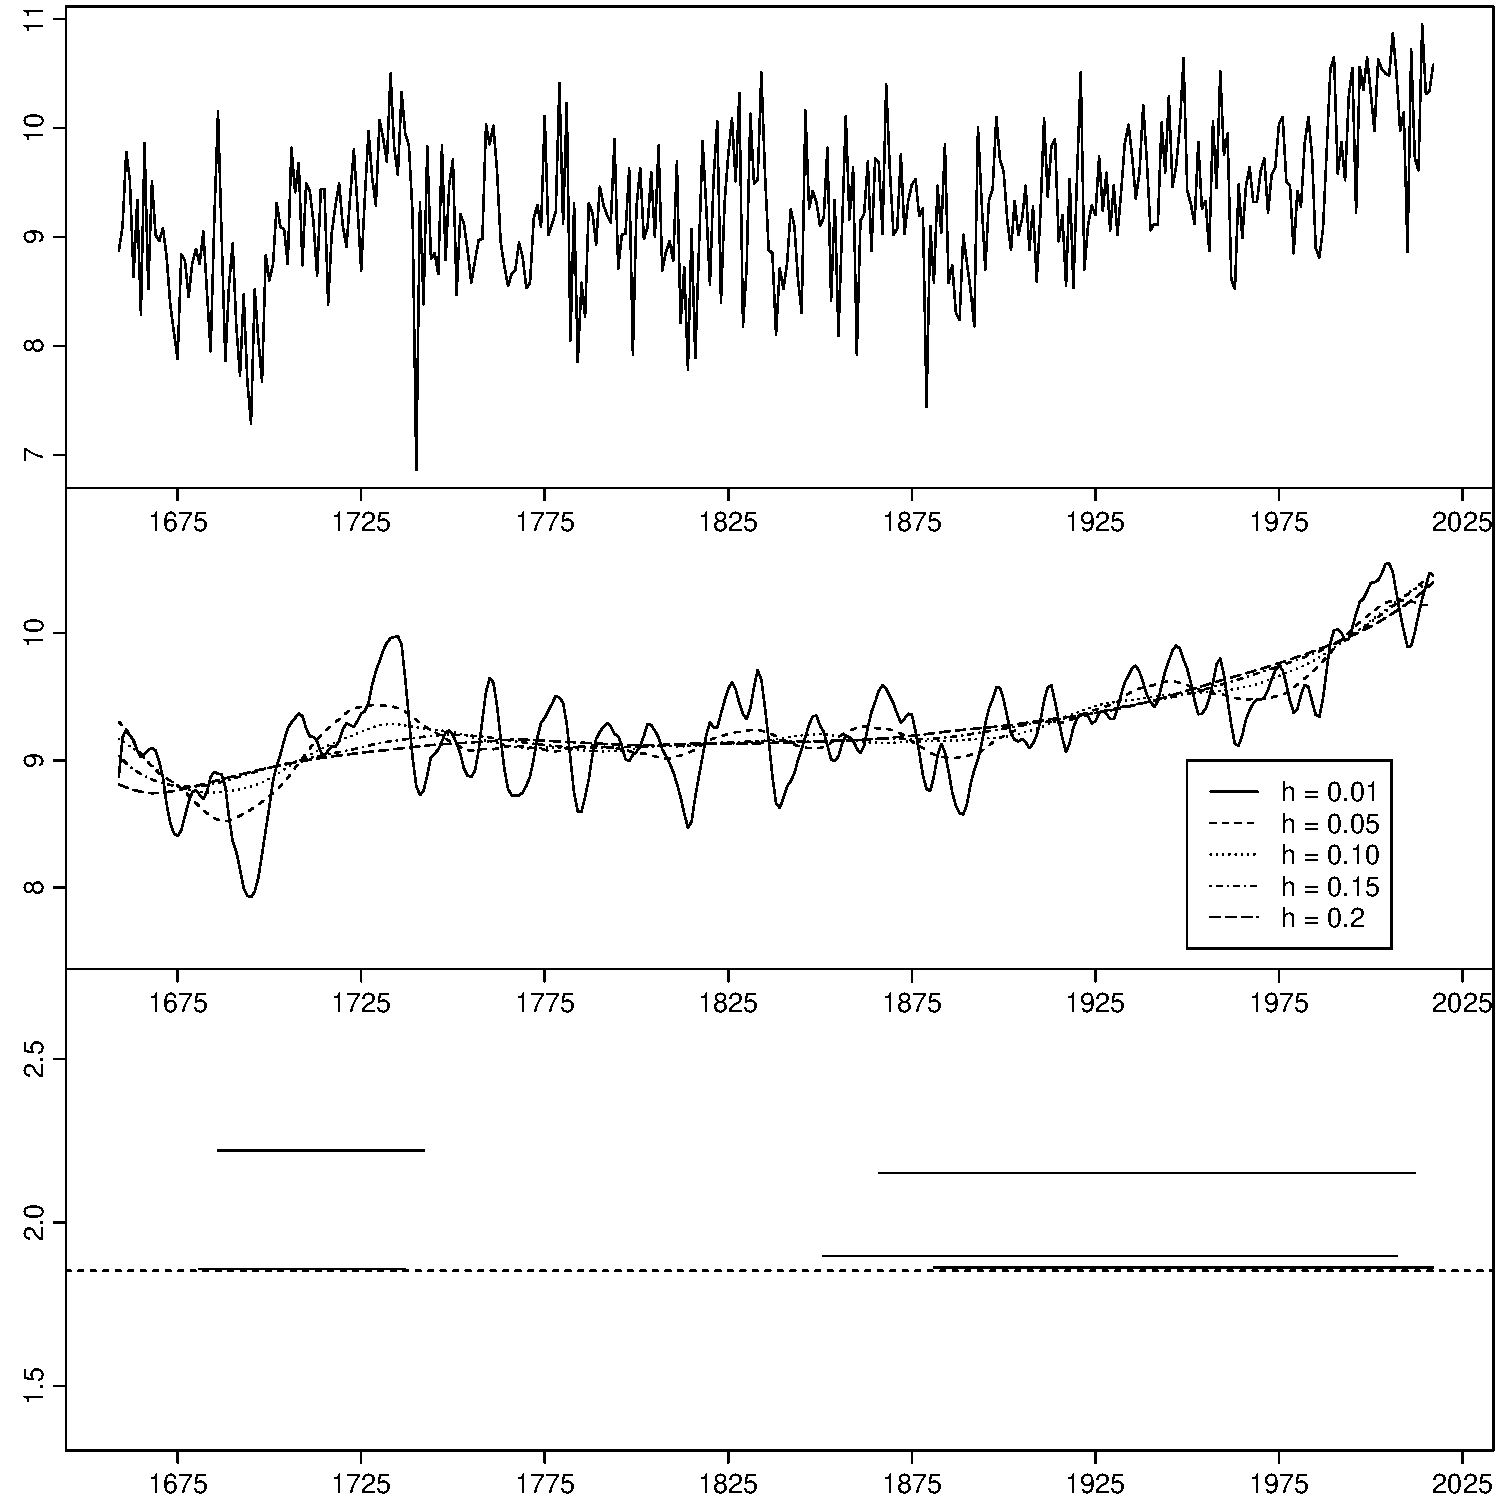
\includegraphics[width=0.8\textwidth]{Plots/threegraphics_testing_constant_method_ll.pdf}
\caption{Summary of the application results for Section \ref{subsec-data-1}. The upper panel shows the Central England mean temperature time series. The middle panel depicts local linear kernel estimates of the time trend for a number of different bandwidths $h$. The lower panel presents the minimal intervals in the set $\Pi_T^+$ produced by the multiscale test. These are $[1681,1737]$, $[1686,1742]$, $[1851,2007]$, $[1866,2012]$ and $[1881,2017]$.}\label{plot-results-app1}
\end{figure}


\enlargethispage{0.2cm}
The analysis of time trends in long temperature records is an important task in climatology. Information on the shape of the trend is needed in order to better understand long-term climate variability. The Central England temperature record is the longest instrumental temperature time series in the world. It is a valuable asset for analysing climate variability over the last few hundred years. The data is publicly available on the webpage of the UK Met Office. A detailed description of the data can be found in \cite{Parker1992}. For our analysis, we use the dataset of yearly mean temperatures which consists of $T=359$ observations covering the years from $1659$ to $2017$. We assume that the data follow the nonparametric trend model 
\[ Y_t = m\Big(\frac{t}{T}\Big) + \varepsilon_t, \]
where $m$ is the unknown time trend of interest. The error process $\{ \varepsilon_t \}$ is supposed to have the AR(1) structure $\varepsilon_t = a \varepsilon_{t-1} + \eta_t$, where $\eta_t$ are i.i.d.\ innovations with mean $0$ and variance $\sigma_\eta^2$. As pointed out in \cite{Mudelsee2010} among others, this is the most widely used error model for discrete climate time series. We estimate the parameters $a$ and $\sigma_\eta^2$ as described in Section \ref{subsec-error-var-ar} which yields the estimates $\widehat{a} \approx 0.267$ and $\widehat{\sigma}_\eta^2 \approx 0.35$.


With the help of our multiscale method from Section \ref{sec-test-shape}, we test the null hypothesis $H_0: m^\prime = 0$, that is, the hypothesis that $m$ is constant. To do so, we set the significance level to $\alpha = 0.05$ and implement the test in exactly the same way as in the simulations of Section \ref{sec-sim}. The results are presented in Figure \ref{plot-results-app1}. The upper panel shows the raw temperature time series, whereas the middle panel depicts local linear kernel estimates of the trend $m$ for different bandwidths $h$. As one can see, the shape of the estimated time trend strongly differs with the chosen bandwidth. When the bandwidth is small, there are many local increases and decreases in the estimated trend. When the bandwidth is large, most of these local variations get smoothed out. Hence, by themselves, the nonparametric fits do not give much information on whether the trend $m$ is increasing or decreasing in certain time regions. 


Our multiscale test provides this kind of information, which is summarized in the lower panel of Figure \ref{plot-results-app1}. The plot depicts the minimal intervals contained in the set $\Pi_T^+$ which is defined in Section \ref{subsec-test-shape-theo}. The set of intervals $\Pi_T^-$ is empty in the present case. The height at which a minimal interval $I_{u,h} = [u-h,u+h] \in \Pi_t^+$ is plotted indicates the value of the corresponding (additively corrected) test statistic $\widehat{\psi}^\prime_T(u,h) / \widehat{\sigma} - \lambda(h)$. The dashed line specifies the critical value $q_T^\prime(\alpha)$, where $\alpha = 0.05$ as already mentioned above. According to Proposition \ref{prop-test-shape-2}, we can make the following simultaneous confidence statement about the collection of minimal intervals in $\Pi_T^+$. We can claim, with confidence of about $95\%$, that the trend function $m$ has some increase on each minimal interval. More specifically, we can claim with this confidence that there has been some upward movement in the trend both in the period from around $1680$ to $1740$ and in the period from about $1880$ onwards. Hence, our test in particular provides evidence that there has been some warming trend in the period over approximately the last $140$ years. On the other hand, as the set $\Pi_T^-$ is empty, there is no evidence of any downward movement of the trend.  


\subsection{Analysis of UK weather station data}\label{subsec-data-2} 


\begin{figure}[t]
\centering
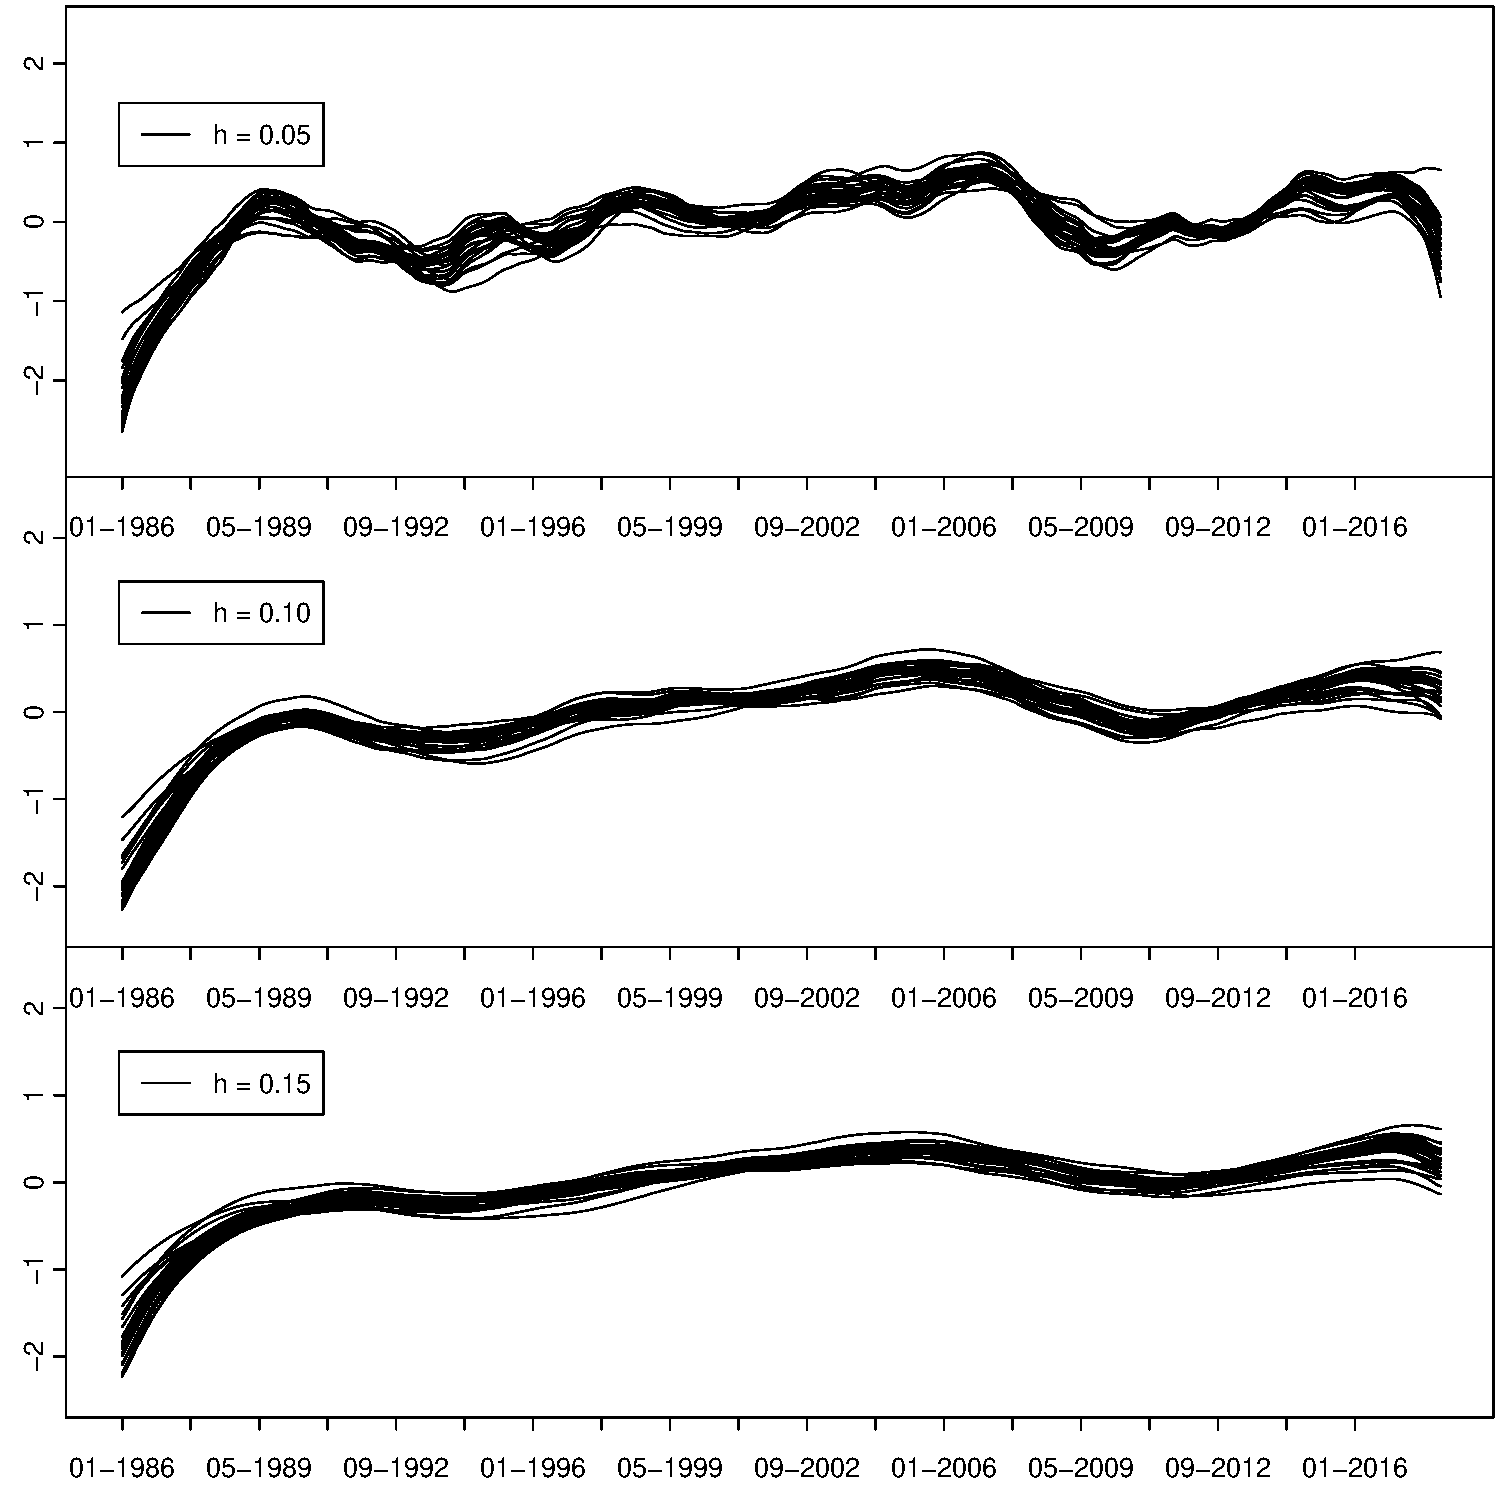
\includegraphics[width=0.8\textwidth]{Plots/stations_data.pdf}
\vspace{0.2cm}
\caption{Local linear kernel estimates of the $n=25$ time trends from the application of Section \ref{subsec-data-2}. Each panel shows the estimates for a different bandwidth $h$.}\label{plot-results-app2}
\end{figure}


To illustrate our test method from Section \ref{sec-test-equality}, we examine a dataset of monthly mean temperatures from $34$ different UK weather stations. The data are publicly available on the webpage of the UK Met Office. We use a subset of $25$ stations for which data are available over the time span from $1986$ to $2017$. We thus observe a time series $\mathcal{Y}_i = \{Y_{it}: 1 \le t \le T \}$ of length $T = 386$ for each station $i \in \{1,\ldots,25\}$. The time series $\mathcal{Y}_i$ is assumed to follow the model 
\begin{equation}\label{model2-app}
Y_{it} = \alpha_i(t) + m_i\Big(\frac{t}{T}\Big) + \varepsilon_{it}, 
\end{equation}
where $m_i$ is an unknown nonparametric time trend and $\alpha_i(t)$ is a month-specific intercept which captures the seasonality pattern in the data. We suppose that $\alpha_i(t) = \alpha_i(t + 12 \ell)$ for any integer $\ell$, that is, we have a different intercept $\alpha_i(k)$ for each month $k = 1,\ldots,12$. The test method and the underlying theory from Section \ref{sec-test-equality} can be easily adapted to model \eqref{model2-app}, which is a slight extension of model \eqref{model2}. The details are provided below. As in Section \ref{subsec-data-1}, the error process $\mathcal{E}_i = \{ \varepsilon_{it}: 1 \le t \le T \}$ is assumed to have the AR(1) structure $\varepsilon_{it} = a_i \varepsilon_{i,t-1} + \eta_{it}$ for each $i$, where $\eta_{it}$ are i.i.d.\ innovations with mean zero.  


We aim to test whether the time trend $m_i$ is the same at each of the $25$ weather stations. In other words, we want to test the null hypothesis $H_0: m_1 = \ldots = m_n$ with $n = 25$ in model \eqref{model2-app}. To do so, we apply the multiscale test from Section \ref{sec-test-equality} with two minor modifications: (i) We define $\widehat{Y}_{it} = Y_{it} - \widehat{\alpha}_i(t)$, where $\widehat{\alpha}_i(t)$ is an estimator of $\alpha_i(t)$. In particular, we set $\widehat{\alpha}_i(t) = \widehat{\alpha}_i(k)$ for any $t = k + 12 \ell$ with $1 \le k \le 12$ and some $\ell \in \integers$, where $\widehat{\alpha}_i(k) = T_k^{-1} \sum_{t = 1}^T \ind_k(t) Y_{it}$ with $\ind_k(t) = \ind(t = k + \lfloor (t-1)/12 \rfloor \cdot 12)$ and $T_k = \sum_{t=1}^T \ind_k(t)$ for $1 \le k \le 12$. (ii) We define the Gaussian statistic $\Phi_{n,T}$ as in Section \ref{subsec-test-equality-test} with $\phi_{ij,T}(u,h) = \sum_{t=1}^T w_{t,T}(u,h) \{ \widehat{\sigma}_i (Z_{it} - \bar{Z}_i(t)) - \widehat{\sigma}_j (Z_{jt} - \bar{Z}_j(t))\}$, where $\bar{Z}_i(t) = \sum_{k=1}^{12} 1_k(t) \{ T_k^{-1} \sum_{s = 1}^T \ind_k(s) Z_{is} \}$. Apart from these two modifications, the multiscale test is constructed exactly as described in Section \ref{sec-test-equality}. We implement the test in the same way as in the simulations of Section \ref{sec-sim}. 


We are now ready to apply the test procedure to the data. Figure \ref{plot-results-app2} depicts local linear estimates of the trend functions $m_i$ for the $n=25$ different stations. Each panel corresponds to a different bandwidth $h$. As can be seen, for a given bandwidth $h$, the fits look very similar to each other. Visual inspection thus suggests that there are no strong differences between the time trends $m_i$. Our test confirms this impression. It does not reject the null hypothesis at the most common levels $\alpha = 0.01, 0.05, 0.1$. Hence, the test does not provide any evidence for a violation of the null. 


\section*{Appendix}

\def\theequation{A.\arabic{equation}}
\setcounter{equation}{0}
\allowdisplaybreaks[4]


In what follows, we prove the theoretical results from Section \ref{sec-method}. The proofs of the results from Sections \ref{sec-test-shape} and \ref{sec-test-equality} are deferred to the Supplementary Material. Throughout the Appendix, we use the following notation: The symbol $C$ denotes a universal real constant which may take a different value on each occurrence. For $a,b \in \reals$, we write $a_+ = \max \{0,a\}$ and $a \vee b = \max\{a,b\}$. For any set $A$, the symbol $|A|$ denotes the cardinality of $A$. The notation $X \stackrel{\mathcal{D}}{=} Y$ means that the two random variables $X$ and $Y$ have the same distribution. Finally, $f_0(\cdot)$ and $F_0(\cdot)$ denote the density and distribution function of the standard normal distribution, respectively.



\subsection*{Auxiliary results using strong approximation theory}


The main purpose of this section is to prove that there is a version of the multiscale statistic $\widehat{\Phi}_T$ defined in \eqref{Phi-hat-statistic} which is close to a Gaussian statistic whose distribution is known. More specifically, we prove the following result. 
%
%
\begin{propA}\label{propA-strong-approx}
Under the conditions of Theorem \ref{theo-stat}, there exist statistics $\widetilde{\Phi}_T$ for $T = 1,2,\ldots$ with the following two properties: (i) $\widetilde{\Phi}_T$ has the same distribution as $\widehat{\Phi}_T$ for any $T$, and (ii)
\[ \big| \widetilde{\Phi}_T - \Phi_T \big| = o_p \Big( \frac{T^{1/q}}{\sqrt{T h_{\min}}} + \rho_T \sqrt{\log T} \Big), \]
where $\Phi_T$ is a Gaussian statistic as defined in \eqref{Phi-statistic}. 
\end{propA}
%
%
\begin{proof}[\textnormal{\textbf{Proof of Proposition \ref{propA-strong-approx}}}] 
For the proof, we draw on strong approximation theory for stationary processes $\{\varepsilon_t\}$ that fulfill the conditions \ref{C-err1}--\ref{C-err3}. By Theorem 2.1 and Corollary 2.1 in \cite{BerkesLiuWu2014}, the following strong approximation result holds true: On a richer probability space, there exist a standard Brownian motion $\mathbb{B}$ and a sequence $\{ \widetilde{\varepsilon}_t: t \in \naturals \}$ such that $[\widetilde{\varepsilon}_1,\ldots,\widetilde{\varepsilon}_T] \stackrel{\mathcal{D}}{=} [\varepsilon_1,\ldots,\varepsilon_T]$ for each $T$ and 
\begin{equation}\label{eq-strongapprox-dep}
\max_{1 \le t \le T} \Big| \sum\limits_{s=1}^t \widetilde{\varepsilon}_s - \sigma \mathbb{B}(t) \Big| = o\big( T^{1/q} \big) \quad \text{a.s.},  
\end{equation}
where $\sigma^2 = \sum_{k \in \integers} \cov(\varepsilon_0, \varepsilon_k)$ denotes the long-run error variance. To apply this result, we define 
\[ \widetilde{\Phi}_T = \max_{(u,h) \in \mathcal{G}_T} \Big\{ \Big|\frac{\widetilde{\phi}_T(u,h)}{\widetilde{\sigma}}\Big| - \lambda(h) \Big\}, \]
where $\widetilde{\phi}_T(u,h) = \sum\nolimits_{t=1}^T w_{t,T}(u,h) \widetilde{\varepsilon}_t$ and $\widetilde{\sigma}^2$ is the same estimator as $\widehat{\sigma}^2$ with $Y_t = m(t/T) + \varepsilon_t$ replaced by $\widetilde{Y}_t = m(t/T) + \widetilde{\varepsilon}_t$ for $1 \le t \le T$. In addition, we let
\begin{align*}
\Phi_T & = \max_{(u,h) \in \mathcal{G}_T} \Big\{ \Big|\frac{\phi_T(u,h)}{\sigma}\Big| - \lambda(h) \Big\} \\
\Phi_T^{\diamond} & = \max_{(u,h) \in \mathcal{G}_T} \Big\{ \Big|\frac{\phi_T(u,h)}{\widetilde{\sigma}}\Big| - \lambda(h) \Big\} 
\end{align*}
with $\phi_T(u,h) = \sum\nolimits_{t=1}^T w_{t,T}(u,h) \sigma Z_t$ and $Z_t = \mathbb{B}(t) - \mathbb{B}(t-1)$. With this notation, we can write 
\begin{equation}\label{eq-strongapprox-bound1}
\big| \widetilde{\Phi}_T - \Phi_T \big| \le \big| \widetilde{\Phi}_T - \Phi_T^{\diamond} \big| + \big| \Phi_T^{\diamond} - \Phi_T \big| = \big| \widetilde{\Phi}_T - \Phi_T^{\diamond} \big| + o_p \big( \rho_T \sqrt{\log T} \big), 
\end{equation}
where the last equality follows by taking into account that $\phi_T(u,h) \sim \normal(0,\sigma^2)$ for all $(u,h) \in \mathcal{G}_T$, $|\mathcal{G}_T| = O(T^\theta)$ for some large but fixed constant $\theta$ and $\widetilde{\sigma}^2 = \sigma^2 + o_p(\rho_T)$. Straightforward calculations yield that 
\[ \big| \widetilde{\Phi}_T - \Phi_T^{\diamond} \big| \le \widetilde{\sigma}^{-1} \max_{(u,h) \in \mathcal{G}_T} \big| \widetilde{\phi}_T(u,h) - \phi_T(u,h) \big|. \]
Using summation by parts,
%($\sum_{i=1}^n a_i b_i = \sum_{i=1}^{n-1} A_i (b_i - b_{i+1}) + A_n b_n$ with $A_j = \sum_{j=1}^i a_j$) 
we further obtain that 
\begin{align*}
\big| \widetilde{\phi}_T(u,h) - \phi_T(u,h) \big| 
 & \le W_T(u,h) \max_{1 \le t \le T} \Big| \sum\limits_{s=1}^t \widetilde{\varepsilon}_s - \sigma \sum\limits_{s=1}^t \big\{ \mathbb{B}(s) - \mathbb{B}(s-1) \big\} \Big| \\
 & = W_T(u,h) \max_{1 \le t \le T} \Big| \sum\limits_{s=1}^t \widetilde{\varepsilon}_s - \sigma \mathbb{B}(t) \Big|,
\end{align*}
where
\[ W_T(u,h) = \sum\limits_{t=1}^{T-1} |w_{t+1,T}(u,h) - w_{t,T}(u,h)| + |w_{T,T}(u,h)|. \]
Standard arguments show that $\max_{(u,h) \in \mathcal{G}_T} W_T(u,h) = O( 1/\sqrt{Th_{\min}} )$. Applying the strong approximation result \eqref{eq-strongapprox-dep}, we can thus infer that 
\begin{align}
\big| \widetilde{\Phi}_T - \Phi_T^{\diamond} \big| 
 & \le \widetilde{\sigma}^{-1} \max_{(u,h) \in \mathcal{G}_T} \big| \widetilde{\phi}_T(u,h) - \phi_T(u,h) \big| \nonumber \\
 & \le \widetilde{\sigma}^{-1} \max_{(u,h) \in \mathcal{G}_T} W_T(u,h) \max_{1 \le t \le T} \Big| \sum\limits_{s=1}^t \widetilde{\varepsilon}_s - \sigma \mathbb{B}(t) \Big| 
   = o_p \Big( \frac{T^{1/q}}{\sqrt{Th_{\min}}} \Big). \label{eq-strongapprox-bound2}
\end{align}
Plugging \eqref{eq-strongapprox-bound2} into \eqref{eq-strongapprox-bound1} completes the proof.
\end{proof}



\subsection*{Auxiliary results using anti-concentration bounds}


In this section, we establish some properties of the Gaussian statistic $\Phi_T$ defined in \eqref{Phi-statistic}. We in particular show that $\Phi_T$ does not concentrate too strongly in small regions of the form $[x-\delta_T,x+\delta_T]$ with $\delta_T$ converging to zero.  
%
%
\begin{propA}\label{propA-anticon}
Under the conditions of Theorem \ref{theo-stat}, it holds that 
\[ \sup_{x \in \reals} \pr \Big( | \Phi_T - x | \le \delta_T \Big) = o(1), \]
where $\delta_T = T^{1/q} / \sqrt{T h_{\min}} + \rho_T \sqrt{\log T}$.
\end{propA}
%
%
\begin{proof}[\textnormal{\textbf{Proof of Proposition \ref{propA-anticon}}}] 
The main technical tool for proving Proposition \ref{propA-anticon} are anti-concentration bounds for Gaussian random vectors. The following proposition slightly generalizes anti-concentration results derived in \cite{Chernozhukov2015}, in particular Theorem 3 therein. 
\begin{propA}\label{theo-anticon}
Let $(X_1,\ldots,X_p)^\top$ be a Gaussian random vector in $\reals^p$ with $\ex[X_j] = \mu_j$ and $\var(X_j) = \sigma_j^2 > 0$ for $1 \le j \le p$. Define $\overline{\mu} = \max_{1 \le j \le p} |\mu_j|$ together with $\underline{\sigma} = \min_{1 \le j \le p} \sigma_j$ and $\overline{\sigma} = \max_{1 \le j \le p} \sigma_j$. Moreover, set $a_p = \ex[ \max_{1 \le j \le p} (X_j-\mu_j)/\sigma_j ]$ and $b_p = \ex[ \max_{1 \le j \le p} (X_j-\mu_j) ]$. For every $\delta > 0$, it holds that
\[ \sup_{x \in \reals} \pr \Big( \big| \max_{1 \le j \le p} X_j - x \big| \le \delta \Big) \le C \delta \big\{ \overline{\mu} + a_p + b_p + \sqrt{1 \vee \log(\underline{\sigma}/\delta)} \big\}, \]
where $C > 0$ depends only on $\underline{\sigma}$ and $\overline{\sigma}$. 
\end{propA} 
%For the sake of completeness, 
The proof of Proposition \ref{theo-anticon} is provided in the Supplementary Material. To apply Proposition \ref{theo-anticon} to our setting at hand, we introduce the following notation: We write $x = (u,h)$ along with $\mathcal{G}_T = \{ x : x \in \mathcal{G}_T \} = \{x_1,\ldots,x_p\}$, where $p := |\mathcal{G}_T| \le O(T^\theta)$ for some large but fixed $\theta > 0$ by our assumptions. Moreover, for $j = 1,\ldots,p$, we set 
\begin{align*}
X_{2j-1} & = \frac{\phi_T(x_{j1},x_{j2})}{\sigma} - \lambda(x_{j2}) \\
X_{2j} & = -\frac{\phi_T(x_{j1},x_{j2})}{\sigma} - \lambda(x_{j2}) 
\end{align*}
with $x_j = (x_{j1},x_{j2})$. This notation allows us to write
\[ \Phi_T = \max_{1 \le j \le 2p} X_j, \]
where $(X_1,\ldots,X_{2p})^\top$ is a Gaussian random vector with the following properties: (i) $\mu_j := \ex[X_j] = - \lambda(x_{j2})$ and thus $\overline{\mu} = \max_{1 \le j \le 2p} |\mu_j| \le C \sqrt{\log T}$, and (ii) $\sigma_j^2 := \var(X_j) = 1$ for all $j$. Since $\sigma_j = 1$ for all $j$, it holds that $a_{2p} = b_{2p}$. Moreover, as the variables $(X_j - \mu_j)/\sigma_j$ are standard normal, we have that $a_{2p} = b_{2p} \le \sqrt{2 \log (2p)} \le C \sqrt{\log T}$. With this notation at hand, we can apply Proposition \ref{theo-anticon} to obtain that 
\[ \sup_{x \in \reals} \pr \Big( \big| \Phi_T - x \big| \le \delta_T \Big) \le C \delta_T \Big[ \sqrt{\log T} + \sqrt{ \log(1/\delta_T) } \Big] = o(1) \]
with $\delta_T = T^{1/q} / \sqrt{T h_{\min}} + \rho_T \sqrt{\log T}$, which is the statement of Proposition \ref{propA-anticon}.
\end{proof}



\subsection*{Proof of Theorem \ref{theo-stat}}


To prove Theorem \ref{theo-stat}, we make use of the two auxiliary results derived above. By Proposition \ref{propA-strong-approx}, there exist statistics $\widetilde{\Phi}_T$ for $T = 1,2,\ldots$ which are distributed as $\widehat{\Phi}_T$ for any $T \ge 1$ and which have the property that 
\begin{equation}\label{statement-propA-strong-approx}
\big| \widetilde{\Phi}_T - \Phi_T \big| = o_p \Big( \frac{T^{1/q}}{\sqrt{T h_{\min}}} + \rho_T \sqrt{\log T} \Big), 
\end{equation}
where $\Phi_T$ is a Gaussian statistic as defined in \eqref{Phi-statistic}. The approximation result \eqref{statement-propA-strong-approx} allows us to replace the multiscale statistic $\widehat{\Phi}_T$ by an identically distributed version $\widetilde{\Phi}_T$ which is close to the Gaussian statistic $\Phi_T$. In the next step, we show that  
\begin{equation}\label{eq-theo-stat-step2}
\sup_{x \in \reals} \big| \pr(\widetilde{\Phi}_T \le x) - \pr(\Phi_T \le x) \big| = o(1), 
\end{equation}
which immediately implies the statement of Theorem \ref{theo-stat}. For the proof of \eqref{eq-theo-stat-step2}, we use the following simple lemma: 
\begin{lemmaA}\label{lemma1-theo-stat}
Let $V_T$ and $W_T$ be real-valued random variables for $T = 1,2,\ldots$ such that $V_T - W_T = o_p(\delta_T)$ with some $\delta_T = o(1)$. If 
\begin{equation}\label{eq-lemma1-cond}
\sup_{x \in \reals} \pr(|V_T - x| \le \delta_T) = o(1), 
\end{equation}
then 
\begin{equation}\label{eq-lemma1-statement}
\sup_{x \in \reals} \big| \pr(V_T \le x) - \pr(W_T \le x) \big| = o(1). 
\end{equation}
\end{lemmaA}
The statement of Lemma \ref{lemma1-theo-stat} can be summarized as follows: If $W_T$ can be approximated by $V_T$ in the sense that $V_T - W_T = o_p(\delta_T)$ and if $V_T$ does not concentrate too strongly in small regions of the form $[x - \delta_T,x+\delta_T]$ as assumed in \eqref{eq-lemma1-cond}, then the distribution of $W_T$ can be approximated by that of $V_T$ in the sense of \eqref{eq-lemma1-statement}.
\begin{proof}[\textnormal{\textbf{Proof of Lemma \ref{lemma1-theo-stat}}}] 
It holds that 
\begin{align*}
 & \big| \pr(V_T \le x) - \pr(W_T \le x) \big| \\
 & = \big| \ex \big[ 1(V_T \le x) - 1(W_T \le x) \big] \big| \\
 & \le \big| \ex \big[ \big\{ 1(V_T \le x) - 1(W_T \le x) \big\} 1(|V_T - W_T| \le \delta_T) \big] \big| + \big| \ex \big[ 1(|V_T - W_T| > \delta_T) \big] \big| \\
 & \le \ex \big[ 1(|V_T - x| \le \delta_T, |V_T - W_T| \le \delta_T) \big] + o(1) \\
 & \le \pr (|V_T - x| \le \delta_T) + o(1). \qedhere
\end{align*}
\end{proof}
We now apply this lemma with $V_T = \Phi_T$, $W_T = \widetilde{\Phi}_T$ and $\delta_T = T^{1/q} / \sqrt{T h_{\min}} + \rho_T \sqrt{\log T}$: From \eqref{statement-propA-strong-approx}, we already know that $\widetilde{\Phi}_T - \Phi_T = o_p(\delta_T)$. Moreover, by Proposition \ref{propA-anticon}, it holds that 
\begin{equation}\label{statement-propA-anticon}
\sup_{x \in \reals} \pr \Big( | \Phi_T - x | \le \delta_T \Big) = o(1). 
\end{equation}
Hence, the conditions of Lemma \ref{lemma1-theo-stat} are satisfied. Applying the lemma, we obtain \eqref{eq-theo-stat-step2}, which completes the proof of Theorem \ref{theo-stat}.
%Note that with the help of Theorem 2.1 in \cite{DuembgenSpokoiny2001}, we can further show that $\Phi_T = O_p(1)$. Together with \eqref{statement-propA-anticon}, this says that the Gaussian multiscale statistic $\Phi_T$ is asymptotically tight and does not concentrate too strongly in small regions of the form $[x - \delta_T,x + \delta_T]$. Putting everything together, we are now in a position to apply Lemma \ref{lemma1-theo-stat}, which in turn yields \eqref{eq-theo-stat-step2}. This completes the proof of Theorem \ref{theo-stat}. 



\subsection*{Proof of Proposition \ref{prop-test-2}}


Write $\widehat{\psi}_T(u,h) = \widehat{\psi}_T^A(u,h) + \widehat{\psi}_T^B(u,h)$ with $\widehat{\psi}_T^A(u,h) = \sum\nolimits_{t=1}^T w_{t,T}(u,h) \varepsilon_t$ and $\widehat{\psi}_T^B(u,h) = \sum\nolimits_{t=1}^T w_{t,T}(u,h) m_T(\frac{t}{T})$. By assumption, there exists $(u_0,h_0) \in \mathcal{G}_T$ with $[u_0-h_0,u_0+h_0] \subseteq [0,1]$ such that $m_T(w) \ge c_T \sqrt{\log T/(Th_0)}$ for all $w \in [u_0-h_0,u_0+h_0]$. Since the kernel $K$ is symmetric and $u_0 = t/T$ for some $t$, it holds that $S_{T,1}(u_0,h_0) = 0$ and thus 
\[ w_{t,T}(u_0,h_0) = K\Big(\frac{\frac{t}{T}-u_0}{h_0}\Big) \Big/ \Big\{ \sum_{t=1}^T K^2\Big(\frac{\frac{t}{T}-u_0}{h_0}\Big) \Big\}^{1/2} \ge 0. \]
Together with the assumption that $m_T(w) \ge c_T \sqrt{\log T/(Th_0)}$ for all $w \in [u_0-h_0,u_0+h_0]$, this implies that 
\begin{equation}\label{eq1-proof-prop-test-power}
\widehat{\psi}_T^B(u_0,h_0) \ge c_T \sqrt{\frac{\log T}{Th_0}} \sum\limits_{t=1}^T w_{t,T}(u_0,h_0).
\end{equation}
Standard calculations exploiting the Lipschitz continuity of the kernel $K$ show that for any $(u,h) \in \mathcal{G}_T$ and any given natural number $\ell$, 
\begin{equation}\label{eq-riemann-sum}
\Big| \frac{1}{Th} \sum\limits_{t=1}^T K\Big(\frac{\frac{t}{T}-u}{h}\Big) \Big(\frac{\frac{t}{T}-u}{h}\Big)^\ell - \int_0^1 \frac{1}{h} K\Big(\frac{w-u}{h}\Big) \Big(\frac{w-u}{h}\Big)^\ell dw \Big| \le \frac{C}{Th}, 
\end{equation}
where the constant $C$ does not depend on $u$, $h$ and $T$. With the help of \eqref{eq-riemann-sum}, we obtain that for any $(u,h) \in \mathcal{G}_T$ with $[u-h,u+h] \subseteq [0,1]$, 
\begin{equation}\label{eq2-proof-prop-test-power}
\Big| \sum\limits_{t=1}^T w_{t,T}(u,h) - \frac{\sqrt{Th}}{\kappa} \Big| \le \frac{C}{\sqrt{Th}}, 
\end{equation}
where $\kappa = (\int K^2(\varphi)d\varphi)^{1/2}$ and the constant $C$ does once again not depend on $u$, $h$ and $T$. From \eqref{eq2-proof-prop-test-power}, it follows that $\sum\nolimits_{t=1}^T w_{t,T}(u,h) \ge \sqrt{Th} / (2\kappa)$ for sufficiently large $T$ and any $(u,h) \in \mathcal{G}_T$ with $[u-h,u+h] \subseteq [0,1]$. This together with \eqref{eq1-proof-prop-test-power} allows us to infer that 
\begin{equation}\label{eq3-proof-prop-test-power}
\widehat{\psi}_T^B(u_0,h_0) \ge \frac{c_T \sqrt{\log T}}{2 \kappa} 
\end{equation}
for sufficiently large $T$. Moreover, arguments very similar to those for the proof of Proposition \ref{propA-strong-approx} yield that
\begin{equation}\label{eq4-proof-prop-test-power}
\max_{(u,h) \in \mathcal{G}_T} |\widehat{\psi}_T^A(u,h)| = O_p(\sqrt{\log T}). 
\end{equation}
With the help of \eqref{eq3-proof-prop-test-power}, \eqref{eq4-proof-prop-test-power} and the fact that $\lambda(h) \le \lambda(h_{\min}) \le C \sqrt{\log T}$, we finally arrive at 
\begin{align}
\widehat{\Psi}_T 
 & \ge \max_{(u,h) \in \mathcal{G}_T} \frac{|\widehat{\psi}_T^B(u,h)|}{\widehat{\sigma}} - \max_{(u,h) \in \mathcal{G}_T} \Big\{ \frac{|\widehat{\psi}_T^A(u,h)|}{\widehat{\sigma}} + \lambda(h) \Big\} \nonumber \\
 & = \max_{(u,h) \in \mathcal{G}_T} \frac{|\widehat{\psi}_T^B(u,h)|}{\widehat{\sigma}} + O_p(\sqrt{\log T}) \nonumber \\
 & \ge \frac{c_T \sqrt{\log T}}{2 \kappa \widehat{\sigma}} + O_p(\sqrt{\log T}). \label{eq5-proof-prop-test-power}
\end{align}  
Since $q_T(\alpha) = O(\sqrt{\log T})$ for any fixed $\alpha \in (0,1)$, \eqref{eq5-proof-prop-test-power} immediately implies that $\pr(\widehat{\Psi}_T \le q_T(\alpha)) = o(1)$. 



\subsection*{Proof of Proposition \ref{prop-test-3}}

 
The statement of Proposition \ref{prop-test-3} is a consequence of the following observation: For all $(u,h) \in \mathcal{G}_T$ with 
\[ \Big|\frac{\widehat{\psi}_T(u,h) - \ex \widehat{\psi}_T(u,h)}{\widehat{\sigma}}\Big| - \lambda(h) \le q_T(\alpha) \quad \text{and} \quad \Big|\frac{\widehat{\psi}_T(u,h)}{\widehat{\sigma}}\Big| - \lambda(h) > q_T(\alpha), \]
it holds that $\ex[\widehat{\psi}_T(u,h)] \ne 0$, which in turn implies that $m(v) \ne 0$ for some $v \in I_{u,h}$. From this observation, we can infer the following: On the event 
\[ \big\{ \widehat{\Phi}_T \le q_T(\alpha) \big\} = \Big\{ \max_{(u,h) \in \mathcal{G}_T} \Big( \Big|\frac{\widehat{\psi}_T(u,h) - \ex \widehat{\psi}_T(u,h)}{\widehat{\sigma}}\Big| - \lambda(h) \Big) \le q_T(\alpha) \Big\}, \]
it holds that for all $(u,h) \in \mathcal{A}_T$, 
$m(v) \ne 0$ for some $v \in I_{u,h}$. Hence, we obtain that 
\[ \big\{ \widehat{\Phi}_T \le q_T(\alpha) \big\} \subseteq E_T. \]
As a result, we arrive at  
\[ \pr(E_T) \ge \pr \big(  \widehat{\Phi}_T \le q_T(\alpha) \big) = (1-\alpha) + o(1), \]
where the last equality holds by Theorem \ref{theo-stat}.




\newpage
\bibliographystyle{ims}
{\small
\setlength{\bibsep}{0.55em}
\bibliography{../Paper/bibliography}}



\end{document}
